% =====================================================================
%  PROYEK LAPORAN MIKROKONTROLER
%  Kompilasi: pdflatex main.tex (2x)  atau  latexmk -pdf main.tex
% =====================================================================
\documentclass[12pt,a4paper,oneside]{book}

\usepackage[utf8]{inputenc}
\usepackage[T1]{fontenc}
% Bahasa Indonesia (jika paket babel-indonesian tidak ada, label diganti manual)
\IfFileExists{indonesian.ldf}{\usepackage[indonesian]{babel}}{%
  \usepackage[english]{babel}
  \AtBeginDocument{%
    \renewcommand{\contentsname}{Daftar Isi}
    \renewcommand{\listfigurename}{Daftar Gambar}
    \renewcommand{\listtablename}{Daftar Tabel}
    \renewcommand{\figurename}{Gambar}
    \renewcommand{\tablename}{Tabel}
    \renewcommand{\refname}{Daftar Pustaka}}}
\IfFileExists{lmodern.sty}{\usepackage{lmodern}}{}
\usepackage[top=3cm,bottom=2.5cm,left=3cm,right=2.5cm]{geometry}
\usepackage{graphicx}
\usepackage{xcolor}
\usepackage{booktabs,array,tabularx}
\usepackage{amsmath}
\usepackage{siunitx}
\sisetup{output-decimal-marker={,}}
\usepackage{float}
\usepackage{caption}
\usepackage{fancyhdr}
\usepackage{listings}
\usepackage{tikz}
\usetikzlibrary{positioning}
\usepackage{pgfplots}
\pgfplotsset{compat=1.18}
\usepackage[american]{circuitikz}
\usepackage{setspace}
\usepackage{tcolorbox}
\usepackage[hidelinks]{hyperref}
\usepackage{tikz}
\usetikzlibrary{shapes.geometric, arrows.meta, positioning, shadows, calc}
\setstretch{1.15}
\setlength{\emergencystretch}{3em}
\usepackage{wrapfig}
\usepackage{graphicx}
\usepackage{microtype}
\usepackage{tabularx}
\usepackage{booktabs}

% ---------- Gaya kode (Arduino/C++) ----------
\definecolor{kode-bg}{gray}{0.96}
\definecolor{kode-kom}{rgb}{0.0,0.5,0.2}
\definecolor{kode-kunci}{rgb}{0.0,0.2,0.7}
\lstdefinestyle{arduino}{
  language=C++, backgroundcolor=\color{kode-bg},
  basicstyle=\ttfamily\small, keywordstyle=\color{kode-kunci}\bfseries,
  commentstyle=\color{kode-kom}\itshape, numbers=left,
  numberstyle=\tiny\color{gray}, frame=single, rulecolor=\color{gray!50},
  breaklines=true, tabsize=2, showstringspaces=false,
  xleftmargin=1.5em, framexleftmargin=1.5em
}
\lstset{style=arduino}
\renewcommand{\lstlistingname}{Kode}

% ---------- Header & footer ----------
\setlength{\headheight}{14.5pt}
\pagestyle{fancy}
\fancyhf{}
\fancyhead[L]{\small\judulpendek}
\fancyhead[R]{\small\namafg}
\fancyfoot[C]{\thepage}
\renewcommand{\headrulewidth}{0.4pt}
\fancypagestyle{plain}{\fancyhf{}\fancyfoot[C]{\thepage}\renewcommand{\headrulewidth}{0pt}}

% ---------- Penomoran: bagian A, B, C, ... di dalam bab ----------
\renewcommand{\thesection}{\Alph{section}}
\renewcommand{\thesubsection}{\thesection.\arabic{subsection}}


% =====================================================================
%  >>> ISI INFORMASI COVER DI SINI <<<\
% =====================================================================
\newif\ifdengancover \dengancovertrue  % ganti \dengancoverfalse bila cover tidak diperlukan
% =====================================================================
%  INFORMASI COVER -- edit file ini saja
% =====================================================================
\newcommand{\judul}{Eksplorasi Sensor dan Actuator}
\newcommand{\judulpendek}{Sensor \& Actuator}
\newcommand{\subjudul}{Kontrol Deteksi Gas dan Udara}
\newcommand{\jenisdokumen}{MATERI PEMBELAJARAN -- SENSOR \& ACTUATOR}
\newcommand{\matakuliah}{Sistem Tertanam -- Gasal 2026/2027}
\newcommand{\nomortugas}{Tugas Focus Group Discussion}

% Penulis (pisahkan baris dengan \\ )
\newcommand{\penulis}{%
  Muh. Syarief Mulyadi \quad (NPM 2206031353)\\
  Humam Al Labib \quad (NPM 220608175)}

\newcommand{\dosen}{Prof. Dr. Ir. Petrus Mursanto, M.Sc.}
\newcommand{\kelompok}{Focus Group 1}
\newcommand{\namafg}{Focus Group 1}
\newcommand{\institusi}{Universitas Indonesia}
\newcommand{\fakultas}{Fakultas Ilmu Komputer}
\newcommand{\kota}{Depok}
\newcommand{\tahun}{2026}

% Logo: letakkan file di folder images/ lalu ubah nama di bawah.
% Jika file tidak ditemukan, kotak placeholder akan ditampilkan.
\newcommand{\logofile}{images/logo.png}
\newcommand{\logowidth}{4cm}

% Informasi tambahan (opsional, boleh dikosongkan: \newcommand{\infotambahan}{})
% \newcommand{\infotambahan}{%
%   Tanggal praktikum: 6 Oktober 2026\\
%   Laboratorium: Lab. Sistem Digital}
\newcommand{\infotambahan}{}

% ---------- Tautan repositori bersama (luaran ke-3) ----------
\newcommand{\repourl}{https://github.com/organisasi/fg1-repo}
\newcommand{\wokwiurl}{https://wokwi.com/projects/000000000}
\newcommand{\videourl}{https://youtu.be/xxxxxxxxxxx}
\newcommand{\slideurl}{https://drive.google.com/xxxxxxxx}


\begin{document}

\hypersetup{pageanchor=false}
\ifdengancover % Halaman sampul -- tidak perlu diedit (gunakan cover-info.tex)
\begin{titlepage}
  \thispagestyle{empty}
  \centering
  \vspace*{0.5cm}

  {\large\bfseries\jenisdokumen\par}
  \vspace{0.4cm}
  {\normalsize\matakuliah\par}
  \vspace{1.2cm}

  \IfFileExists{\logofile}{%
    \includegraphics[width=\logowidth]{\logofile}%
  }{%
    \fbox{\parbox[c][\logowidth][c]{\logowidth}{\centering\small\color{gray}%
      Letakkan logo di\\ \texttt{\detokenize{images/logo.png}}}}%
  }
  \vspace{1.2cm}

  \rule{\textwidth}{1.2pt}\\[0.5cm]
  {\LARGE\bfseries\judul\par}
  \vspace{0.3cm}
  {\large\itshape\subjudul\par}
  \rule{\textwidth}{1.2pt}

  \vspace{1.5cm}
  {\normalsize Disusun oleh:\par}
  \vspace{0.3cm}
  {\normalsize\bfseries\kelompok\par}
  \vspace{0.2cm}
  {\normalsize\penulis\par}

  \vspace{0.8cm}
  {\normalsize Dosen Pengampu:\\ \textbf{\dosen}\par}

  \ifx\infotambahan\empty\else
    \vspace{0.8cm}
    {\small\infotambahan\par}
  \fi

  \vfill
  {\large\bfseries\fakultas\par}
  {\large\bfseries\institusi\par}
  {\normalsize\kota, \tahun\par}
\end{titlepage}
 \fi
\hypersetup{pageanchor=true}

\frontmatter
\tableofcontents
\clearpage
\listoffigures
\listoftables
\mainmatter

% Seluruh isi bab ada di bab.tex (dapat di-\input langsung ke buku induk)
% =====================================================================
%  BAB BUKU -- dapat di-\input ke buku induk (butuh paket di main.tex)
% =====================================================================
%\chapter{\judul}
%\label{bab:fg}

\section{Pendahuluan}

\subsection{Latar Belakang}
Sistem tertanam dapat digunakan untuk memantau kondisi lingkungan melalui sensor dan mengendalikan komponen berdasarkan hasil pembacaan tersebut. Salah satu penerapannya adalah sistem kontrol dan deteksi udara serta gas yang memanfaatkan sensor untuk mendeteksi kondisi atau kandungan tertentu di lingkungan.

Dalam FGD ini, pembahasan difokuskan pada eksplorasi sensor, aktuator, dan komponen pendukung yang digunakan dalam sistem kontrol deteksi udara dan gas. Eksplorasi dilakukan untuk memahami prinsip kerja, karakteristik sinyal, serta cara setiap komponen berinteraksi dengan mikrokontroler. Proyek yang dibuat selanjutnya digunakan sebagai eksperimen untuk menerapkan dan membuktikan pemahaman tersebut.

\subsection{Tujuan Pembelajaran}
Setelah mempelajari laporan ini, pembaca diharapkan mampu:
\begin{enumerate}
  \item menjelaskan prinsip kerja setiap sensor, aktuator, dan komponen pendukung;
  \item menjelaskan besaran yang diukur atau dikendalikan oleh setiap komponen;
  \item menjelaskan karakteristik sinyal, pin, catu daya, dan antarmuka komponen;
  \item menjelaskan hubungan komponen dengan fitur mikrokontroler yang digunakan;
  \item menghubungkan prinsip kerja dengan rangkaian dan program sederhana;
  \item merancang eksperimen sederhana beserta rangkaiannya untuk membuktikan pemahaman terhadap komponen;
\end{enumerate}

\subsection{Ruang Lingkup}
Pembahasan mencakup komponen yang dieksplorasi oleh Focus Group, mikrokontroler
yang digunakan, rangkaian fisik, code program, serta eksperimen pembuktian.

\subsection{Daftar Komponen yang Dieksplorasi}
\begin{table}[H]
\centering
\caption{Daftar komponen yang menjadi objek eksplorasi}
\begin{tabularx}{\textwidth}{@{}clX@{}}
\toprule
No. & Komponen & Peran dalam eksplorasi \\
\midrule
1 & DHT22 & Sensor/aktuator/komponen pendukung yang dieksplorasi \\
2 & MQ-135 & Sensor/aktuator/komponen pendukung yang dieksplorasi \\
3 & MQ-2 & Sensor/aktuator/komponen pendukung yang dieksplorasi \\
4 & HC-SR501 & Sensor/aktuator/komponen pendukung yang dieksplorasi \\
5 & FC-51 & Sensor/aktuator/komponen pendukung yang dieksplorasi \\
6 & JQC-3FF-S-Z & Sensor/aktuator/komponen pendukung yang dieksplorasi \\
7 & SG90 & Sensor/aktuator/komponen pendukung yang dieksplorasi \\
8 & Micro DC Motor 6 \volt &sfsdf \\
\bottomrule
\end{tabularx}
\end{table}

\newpage

\section{Mikrokontroler}
\label{sec:konsep-mikrokontroler}

\begin{wrapfigure}{r}{0.38\textwidth} % 'r' = sisi kanan, 0.38\textwidth = lebar area gambar
	\vspace{-12pt} % Menggeser posisi gambar sedikit ke atas agar sejajar dengan baris pertama teks
	\centering
	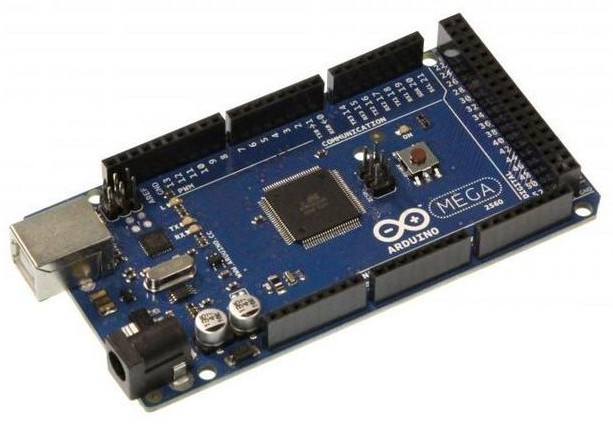
\includegraphics[width=0.36\textwidth]{images/2560.jpg} % Ganti dengan file gambar Anda
	\caption{Ardunio ATmega2560}
	\label{fig:pembuka_mcu}
	\vspace{-10pt} % Mengurangi jarak kosong di bawah caption
\end{wrapfigure}

Bagian ini memberikan landasan konseptual mengenai mikrokontroler sebelum pembahasan masuk ke prinsip kerja masing-masing komponen. Mikrokontroler berperan sebagai pusat pengendalian yang membaca masukan, memproses data, dan menghasilkan keluaran sesuai program. Pemahaman mengenai konsep ini diperlukan agar hubungan antara karakteristik komponen dan fitur mikrokontroler dapat dijelaskan secara teknis.

\par % Memastikan paragraf tersusun rapi sebelum masuk ke subbab berikutnya

\subsection{Pengertian dan Peran Mikrokontroler}
Mikrokontroler adalah sebuah sistem komputer lengkap yang dikemas dalam satu sirkuit terpadu (\textit{Integrated Circuit}/IC). Berbeda dengan mikroprosesor umum (seperti CPU pada PC) yang membutuhkan komponen eksternal terpisah seperti RAM, ROM, dan pengontrol I/O, mikrokontroler telah mengintegrasikan pemroses, memori, dan antarmuka periferal ke dalam satu cip tunggal.

Dalam sistem deteksi udara dan gas pada kegiatan ini, mikrokontroler beroperasi sebagai unit pemroses terpusat (\textit{brain module}). Mikrokontroler bertugas membaca sinyal fisik dari sensor (seperti suhu, gas, dan gerakan), memproses data tersebut berdasarkan algoritma kendali, lalu memberikan instruksi kepada aktuator (seperti penggerak servo, motor DC, atau sakelar relay) untuk merespons kondisi lingkungan secara akurat.

\begin{figure}[H]
	\centering
	\resizebox{\textwidth}{!}{%
		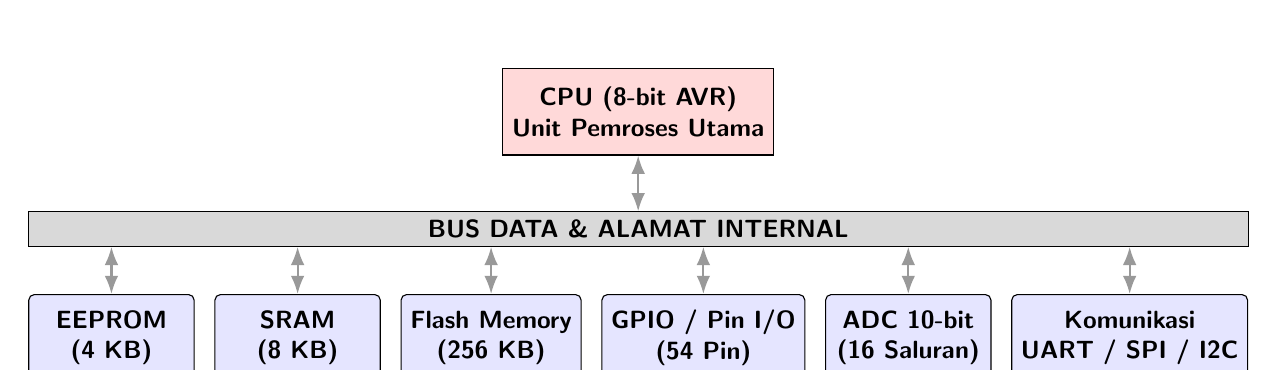
\begin{tikzpicture}[
				node distance=0.6cm and 0.25cm,
				block/.style={rectangle, draw, fill=blue!10, rounded corners=2pt, minimum width=2.1cm, minimum height=1.1cm, align=center, font=\small\sffamily\bfseries},
				core/.style={rectangle, draw, fill=red!15, minimum width=3.2cm, minimum height=1.1cm, align=center, font=\small\sffamily\bfseries},
				arrow/.style={Latex-Latex, thick, draw=gray!80}
			]

			% 1. Buat 6 Blok Bawah Terlebih Dahulu secara Sejajar Horisontal
			\node[block] (eeprom) {EEPROM\\(4 KB)};
			\node[block, right=0.25cm of eeprom] (sram) {SRAM\\(8 KB)};
			\node[block, right=0.25cm of sram] (flash) {Flash Memory\\(256 KB)};
			\node[block, right=0.25cm of flash] (gpio) {GPIO / Pin I/O\\(54 Pin)};
			\node[block, right=0.25cm of gpio] (adc) {ADC 10-bit\\(16 Saluran)};
			\node[block, right=0.25cm of adc] (comm) {Komunikasi\\UART / SPI / I2C};

			% 2. Gambar Bus Abu-Abu Presisi dari Ujung Kiri EEPROM ke Ujung Kanan COMM
			\draw[fill=gray!30, draw=black]
			($(eeprom.north west)+(0, 0.6cm)$) rectangle ($(comm.north east)+(0, 1.05cm)$);

			% Tulis Teks di Tengah Bus
			\path ($(eeprom.north west)!0.5!(comm.north east)+(0, 0.825cm)$)
			node[font=\small\sffamily\bfseries] (bus_text) {BUS DATA \& ALAMAT INTERNAL};

			% Koordinat Sisi Atas dan Bawah Bus untuk Acuan Panah
			\coordinate (bus_south) at ($(eeprom.north west)+(0, 0.6cm)$);
			\coordinate (bus_north) at ($(eeprom.north west)+(0, 1.05cm)$);

			% 3. Buat CPU di Atas Bus (Tepat di Tengah Horisontal)
			\node[core, above=0.7cm of bus_text.north] (cpu) {CPU (8-bit AVR)\\Unit Pemroses Utama};

			% 4. Tarik Panah Hubungan
			\draw[arrow] (cpu.south) -- (cpu.south |- bus_north);
			\draw[arrow] (eeprom.north) -- (eeprom.north |- bus_south);
			\draw[arrow] (sram.north) -- (sram.north |- bus_south);
			\draw[arrow] (flash.north) -- (flash.north |- bus_south);
			\draw[arrow] (gpio.north) -- (gpio.north |- bus_south);
			\draw[arrow] (adc.north) -- (adc.north |- bus_south);
			\draw[arrow] (comm.north) -- (comm.north |- bus_south);

		\end{tikzpicture}%
	}
	\caption{Diagram blok arsitektur dasar mikrokontroler ATmega2560.}
	\label{fig:mcu_architecture}
\end{figure}

\subsection{General Purpose Input/Output (GPIO) dan Logika Digital}

Pin \textit{General Purpose Input/Output} (GPIO) merupakan antarmuka diskrit pada mikrokontroler yang arah operasinya dikonfigurasi via perangkat lunak melalui \textit{Data Direction Register} (DDR). Saat memproses sinyal biner, GPIO bekerja pada dua taraf logika:
\begin{itemize}
    \item \textbf{Logika HIGH (1):} Sinyal aktif ketika tegangan berada pada ambang atas mendekati $V_{CC}$ ($\approx 5\,\text{V DC}$).
    \item \textbf{Logika LOW (0):} Sinyal non-aktif ketika tegangan berada pada ambang bawah mendekati \textit{Ground} ($0\,\text{V DC}$).
\end{itemize}

\subsubsection{Kondisi Mengambang (\textit{Floating State}) dan Resistor Pembatas}

Saat dikonfigurasi sebagai \textit{input}, gerbang internal GPIO berada pada kondisi impedansi tinggi (\textit{High-Z}, $>100\,\text{M}\Omega$). Jika sakelar atau sensor di luarnya terbuka (\textit{open circuit}), pin masukan terisolasi dari tegangan maupun \textit{Ground}. Kondisi ini membuat pin bertindak seperti antena yang rentan terhadap induksi elektromagnetik dan \textit{noise} lingkungan, sehingga tegangannya berfluktuasi acak antara $0\,\text{V}$ dan $5\,\text{V}$ (\textit{floating state}).

Fluktuasi akibat \textit{floating} dapat memicu interupsi palsu (\textit{glitch}) dan kesalahan logika program. Oleh karena itu, sistem memerlukan kepastian status sinyal saat tidak ada masukan aktif. Kepastian logika ini dicapai melalui teknik \textit{biasing} menggunakan resistor (umumnya $10\,\text{k}\Omega$) dalam dua skema:
\begin{itemize}
    \item \textbf{Resistor \textit{Pull-Up}:} Menghubungkan pin masukan ke $V_{CC}$. Saat sakelar terbuka, pin ditarik ke $V_{CC}$ (\texttt{HIGH}). Ketika sakelar ditutup ke \textit{Ground}, tegangan pin jatuh ke $0\,\text{V}$ (\texttt{LOW}) tanpa menyebabkan hubung singkat.
    \item \textbf{Resistor \textit{Pull-Down}:} Menghubungkan pin masukan ke \textit{Ground}. Saat sakelar terbuka, pin ditarik ke \textit{Ground} (\texttt{LOW}). Ketika sakelar ditutup ke $V_{CC}$, pembacaan pin berubah menjadi \texttt{HIGH}.
\end{itemize}

Pada Arduino Mega 2560 (ATmega2560), setiap pin GPIO telah memiliki \textit{Internal Pull-Up Resistor} ($20\text{--}50\,\text{k}\Omega$) yang dapat diaktifkan melalui register perangkat lunak, sehingga menyederhanakan rangkaian eksternal.

\subsection{ADC dan Pembacaan Sinyal Analog}
\textit{Analog-to-Digital Converter} (ADC) berfungsi mengubah sinyal tegangan kontinu dari sensor analog menjadi nilai digital diskrit. Mikrokontroler ATmega2560 dilengkapi dengan ADC beresolusi $10\text{-bit}$ dan tegangan referensi standar $V_{ref} = 5\,\text{V}$.

Sinyal tegangan masuk $V_{in}$ dikonversi menjadi nilai digital $D_{out}$ bertipe integer ($0$ hingga $2^{10}-1 = 1023$) berdasarkan Persamaan~\eqref{eq:adc_conversion}:

\begin{equation}
	\label{eq:adc_conversion}
	D_{out} = \left\lfloor \frac{V_{in}}{V_{ref}} \times (2^n - 1) \right\rfloor = \left\lfloor \frac{V_{in}}{5\,\text{V}} \times 1023 \right\rfloor
\end{equation}

Sebagai contoh, jika sensor MQ-135 menghasilkan tegangan keluaran analog sebesar $2{,}5\,\text{V}$, maka nilai digital yang dibaca oleh ADC mikrokontroler adalah:
\[
	D_{out} = \left\lfloor \frac{2{,}5\,\text{V}}{5\,\text{V}} \times 1023 \right\rfloor = 511
\]

\subsection{PWM dan Pengendalian Output}
\textit{Pulse Width Modulation} (PWM) adalah teknik untuk menyimulasikan luaran analog menggunakan sinyal digital cepat berfrekuensi tetap. Parameter utama PWM adalah \textit{Duty Cycle}, yaitu rasio durasi sinyal \textit{HIGH} ($t_{on}$) terhadap total periode sinyal ($T$), dirumuskan pada Persamaan~\eqref{eq:duty_cycle}:

\begin{equation}
	\label{eq:duty_cycle}
	\text{Duty Cycle (\%)} = \left( \frac{t_{on}}{T} \right) \times 100\%
\end{equation}

Tegangan efektif rata-rata ($V_{eff}$) yang diterima oleh beban dirumuskan pada Persamaan~\eqref{eq:v_eff}:

\begin{equation}
	\label{eq:v_eff}
	V_{eff} = V_{CC} \times \text{Duty Cycle}
\end{equation}

Ilustrasi bentuk gelombang sinyal PWM pada berbagai variasi \textit{duty cycle} disajikan pada Gambar~\ref{fig:pwm_waveform}.

\begin{figure}[H]
	\centering
	\resizebox{0.85\textwidth}{!}{%
		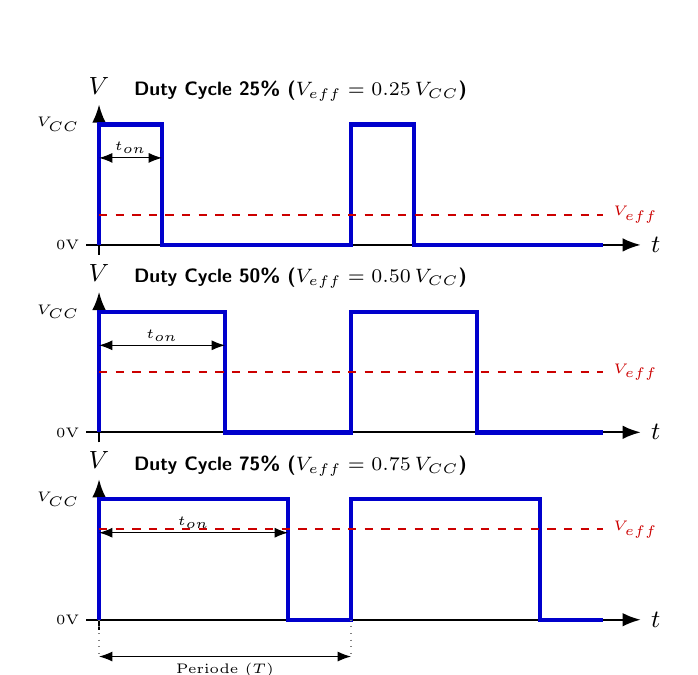
\begin{tikzpicture}[
				xscale=1.6, yscale=0.85,
				signal/.style={ultra thick, blue!80!black},
				avg/.style={dashed, red!80!black, thick}
			]

			% ==================== 1. DUTY CYCLE 25% ====================
			\begin{scope}[shift={(0,5.6)}]
				% Judul Tanpa Label A/B/C
				\node[anchor=west, font=\scriptsize\sffamily\bfseries] at (0.2, 2.3) {Duty Cycle 25\% ($V_{eff} = 0.25 \, V_{CC}$)};

				% Sumbu Koordinat
				\draw[-Latex, thick] (-0.1,0) -- (4.3,0) node[right, font=\small\sffamily] {$t$};
				\draw[-Latex, thick] (0,-0.15) -- (0,2.1) node[above, font=\small\sffamily] {$V$};

				% Label Sumbu Tegangan (Presisi di Samping Sumbu Y)
				\node[anchor=east, font=\tiny] at (-0.08, 1.8) {$V_{CC}$};
				\node[anchor=east, font=\tiny] at (-0.08, 0) {$0\text{V}$};

				% Gelombang Pulsa
				\draw[signal] (0,0) -- (0,1.8) -- (0.5,1.8) -- (0.5,0) -- (2,0) -- (2,1.8) -- (2.5,1.8) -- (2.5,0) -- (4,0);

				% Garis Rata-rata Veff
				\draw[avg] (0,0.45) -- (4,0.45) node[right, font=\tiny\sffamily, red!80!black] {$V_{eff}$};

				% Indikator Ton
				\draw[Latex-Latex, thin] (0,1.3) -- (0.5,1.3) node[midway, above=-2pt, font=\tiny] {$t_{on}$};
			\end{scope}

			% ==================== 2. DUTY CYCLE 50% ====================
			\begin{scope}[shift={(0,2.8)}]
				% Judul Tanpa Label A/B/C
				\node[anchor=west, font=\scriptsize\sffamily\bfseries] at (0.2, 2.3) {Duty Cycle 50\% ($V_{eff} = 0.50 \, V_{CC}$)};
				% Sumbu Koordinat
				\draw[-Latex, thick] (-0.1,0) -- (4.3,0) node[right, font=\small\sffamily] {$t$};
				\draw[-Latex, thick] (0,-0.15) -- (0,2.1) node[above, font=\small\sffamily] {$V$};

				% Label Sumbu Tegangan
				\node[anchor=east, font=\tiny] at (-0.08, 1.8) {$V_{CC}$};
				\node[anchor=east, font=\tiny] at (-0.08, 0) {$0\text{V}$};

				% Gelombang Pulsa
				\draw[signal] (0,0) -- (0,1.8) -- (1,1.8) -- (1,0) -- (2,0) -- (2,1.8) -- (3,1.8) -- (3,0) -- (4,0);

				% Garis Rata-rata Veff
				\draw[avg] (0,0.9) -- (4,0.9) node[right, font=\tiny\sffamily, red!80!black] {$V_{eff}$};

				% Indikator Ton
				\draw[Latex-Latex, thin] (0,1.3) -- (1,1.3) node[midway, above=-2pt, font=\tiny] {$t_{on}$};
			\end{scope}

			% ==================== 3. DUTY CYCLE 75% ====================
			\begin{scope}[shift={(0,0)}]
				% Judul Tanpa Label A/B/C
				\node[anchor=west, font=\scriptsize\sffamily\bfseries] at (0.2, 2.3) {Duty Cycle 75\% ($V_{eff} = 0.75 \, V_{CC}$)};

				% Sumbu Koordinat
				\draw[-Latex, thick] (-0.1,0) -- (4.3,0) node[right, font=\small\sffamily] {$t$};
				\draw[-Latex, thick] (0,-0.15) -- (0,2.1) node[above, font=\small\sffamily] {$V$};


				% Label Sumbu Tegangan
				\node[anchor=east, font=\tiny] at (-0.08, 1.8) {$V_{CC}$};
				\node[anchor=east, font=\tiny] at (-0.08, 0) {$0\text{V}$};

				% Gelombang Pulsa
				\draw[signal] (0,0) -- (0,1.8) -- (1.5,1.8) -- (1.5,0) -- (2,0) -- (2,1.8) -- (3.5,1.8) -- (3.5,0) -- (4,0);

				% Garis Rata-rata Veff
				\draw[avg] (0,1.35) -- (4,1.35) node[right, font=\tiny\sffamily, red!80!black] {$V_{eff}$};

				% Indikator Ton
				\draw[Latex-Latex, thin] (0,1.3) -- (1.5,1.3) node[midway, above=-2pt, font=\tiny] {$t_{on}$};

				% Indikator Periode T
				\draw[Latex-Latex, thin] (0,-0.55) -- (2,-0.55) node[midway, below=-1pt, font=\tiny] {Periode ($T$)};
				\draw[dotted, gray] (2,0) -- (2,-0.55);
				\draw[dotted, gray] (0,0) -- (0,-0.55);
			\end{scope}

		\end{tikzpicture}%
	}
	\caption{Bentuk gelombang sinyal PWM pada variasi \textit{duty cycle} 25\%, 50\%, dan 75\% beserta tegangan efektif rata-ratanya ($V_{eff}$).}
	\label{fig:pwm_waveform}
\end{figure}

PWM digunakan secara mendasar dalam eksperimen ini untuk mengendalikan posisi sudut servo SG90 (lebar pulsa $1\text{--}2\,\text{ms}$) serta mengatur kecepatan putar Motor DC melalui rasio tegangannya.

\subsection{Timer dan Interrupt}
\begin{itemize}
	\item \textbf{Timer/Counter:} Periferal independen dari CPU yang menghitung pulsa detak mikrokontroler. Timer memungkinkan pewaktuan presisi tanpa membebani CPU (\textit{non-blocking delay}).
	\item \textbf{Interrupt:} Mekanisme yang menghentikan sementara eksekusi program utama (\textit{main loop}) ketika terjadi peristiwa tertentu (misalnya perubahan logika pin atau limpahan timer/overflow). CPU akan melompat ke fungsi khusus yang disebut \textit{Interrupt Service Routine} (ISR), mengeksekusinya, lalu kembali ke alur program utama. Mekanisme ini sangat krusial untuk menangani interupsi darurat dari sensor krisis seperti deteksi gas berlebih atau sensor pergerakan PIR.
\end{itemize}

\subsection{Antarmuka Komunikasi}
Mikrokontroler memanfaatkan beberapa protokol komunikasi serial terstandar:
\begin{itemize}
	\item \textbf{UART (\textit{Universal Asynchronous Receiver-Transmitter}):} Komunikasi asinkron titik-ke-titik menggunakan dua jalur sinyal ($TX$ dan $RX$). Digunakan untuk komunikasi data antara Arduino Mega dan PC melalui pengonversi USB-to-Serial.
	\item \textbf{I2C (\textit{Inter-Integrated Circuit}):} Komunikasi sinkron berbasis bus menggunakan dua jalur ($SDA$ untuk data, $SCL$ untuk detak). Memungkinkan hubungan dengan banyak periferal secara paralel menggunakan alamat memori unik.
	\item \textbf{SPI (\textit{Serial Peripheral Interface}):} Komunikasi sinkron berkecepatan tinggi berbasis penuh dupleks (\textit{full-duplex}) yang menggunakan jalur $MOSI$, $MISO$, $SCLK$, dan $SS$.
\end{itemize}

\subsection{Catu Daya dan Level Tegangan}
Papan Arduino Mega 2560 beroperasi pada level logika $5\,\text{V}$. Catu daya utama disediakan via kabel USB ($5\,\text{V}$) atau catu daya eksternal melalui jack DC ($7\text{--}12\,\text{V}$) yang diturunkan oleh regulator terpasang (\textit{on-board voltage regulator}).

Pertimbangan catu daya meliputi batasan arus maksimum tiap pin GPIO ($\pm 20\,\text{mA}$) serta kapasitas daya maksimum regulator. Komponen aktuator bernilai arus tinggi seperti Motor DC dan Modul Relay ditenagai melalui catu eksternal terpisah guna menghindari fluktuasi tegangan yang dapat memicu fenomena \textit{reset} otomatis pada mikrokontroler.

\subsection{Proses Pemrograman, \textit{Flashing}, dan Alur Memori}
Proses memasukkan instruksi program dari komputer (\textit{host}) ke dalam Flash Memory mikrokontroler melibatkan beberapa tahapan transmisi data dan partisi memori, yang diilustrasikan pada Gambar~\ref{fig:flashing_flow}.

\begin{figure}[H]
	\centering
	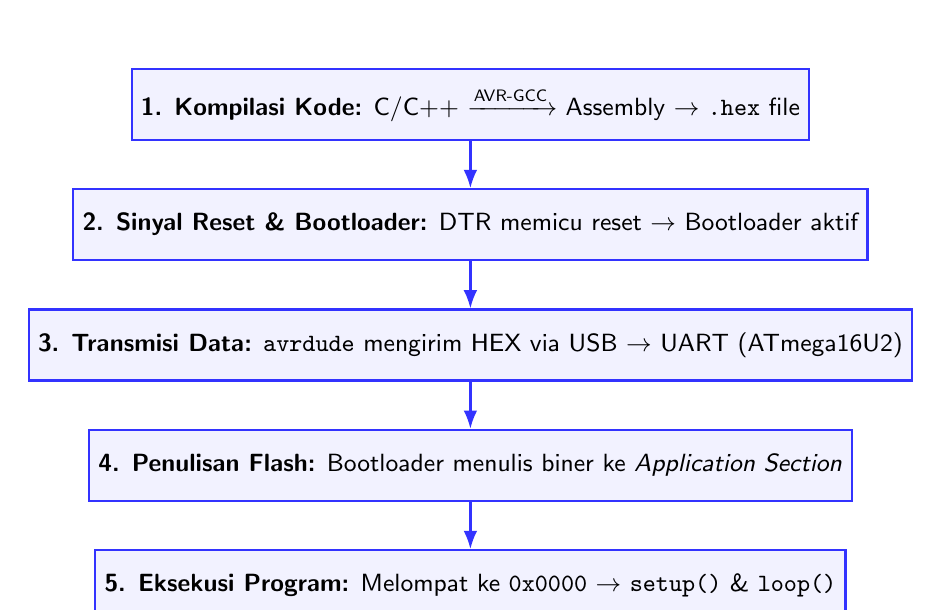
\begin{tikzpicture}[
			node distance=1cm,
			stepblock/.style={rectangle, draw=blue!80, fill=blue!5, thick, minimum width=8.5cm, minimum height=0.9cm, align=left, font=\small\sffamily},
			arrow/.style={-Latex, thick, draw=blue!80}
		]

		\node[stepblock] (step1) {\textbf{1. Kompilasi Kode:} C/C++ $\xrightarrow{\text{AVR-GCC}}$ Assembly $\rightarrow$ \texttt{.hex} file};
		\node[stepblock, below=0.6cm of step1] (step2) {\textbf{2. Sinyal Reset \& Bootloader:} DTR memicu reset $\rightarrow$ Bootloader aktif};
		\node[stepblock, below=0.6cm of step2] (step3) {\textbf{3. Transmisi Data:} \texttt{avrdude} mengirim HEX via USB $\rightarrow$ UART (ATmega16U2)};
		\node[stepblock, below=0.6cm of step3] (step4) {\textbf{4. Penulisan Flash:} Bootloader menulis biner ke \textit{Application Section}};
		\node[stepblock, below=0.6cm of step4] (step5) {\textbf{5. Eksekusi Program:} Melompat ke \texttt{0x0000} $\rightarrow$ \texttt{setup()} \& \texttt{loop()}};

		\draw[arrow] (step1) -- (step2);
		\draw[arrow] (step2) -- (step3);
		\draw[arrow] (step3) -- (step4);
		\draw[arrow] (step4) -- (step5);

	\end{tikzpicture}
	\caption{Alur proses kompilasi, transmisi serial, dan penulisan memori (\textit{flashing}).}
	\label{fig:flashing_flow}
\end{figure}

Penjelasan rincian tahapan alur di atas adalah sebagai berikut:
\begin{enumerate}
	\item \textbf{Kompilasi Kode (\textit{Compilation}):} Perangkat lunak pengembang merubah kode sumber berbasis C/C++ menjadi instruksi mesin dalam bentuk berkas \textit{Intel HEX}.
	\item \textbf{Mekanisme \textit{Bootloader}:} Saat sinyal DTR dialirkan melalui saluran USB, papan akan mereset ATmega2560. Kode \textit{Bootloader} yang berada pada area memori atas (\textit{Bootloader Section}) langsung mengambil alih kendali CPU.
	\item \textbf{Proses \textit{Flashing} via UART:} \textit{Bootloader} menerima data \textit{Intel HEX} yang ditransmisikan secara serial melalui antarmuka UART.
	\item \textbf{Penulisan Memori Flash:} Data biner dituliskan baris demi baris ke dalam \textit{Application Flash Section} secara permanen.
	\item \textbf{Inisialisasi Eksekusi Memori:} Setelah verifikasi sukses, \textit{Bootloader} mengarahkan \textit{Program Counter} (PC) ke alamat \texttt{0x0000} (\textit{Reset Vector}) untuk mulai mengeksekusi fungsi utama program.
\end{enumerate}

\subsection{Alur Data pada Sistem}
Secara menyeluruh, alur kerja sistem kontrol berbasis mikrokontroler dibagi menjadi tiga tahap utama:
\[
	\text{Sensor (Input)} \longrightarrow \text{Pemrosesan Data (Mikrokontroler)} \longrightarrow \text{Aktuator (Output)}
\]
Sinyal analog/digital dari sensor dibaca melalui GPIO atau ADC, diolah menggunakan logika komputasi pada CPU, kemudian perintah dialirkan kembali dalam bentuk sinyal digital atau PWM untuk memicu aksi pada aktuator.


\subsection{Spesifikasi Mikrokontroler yang Digunakan}
Spesifikasi teknis papan pengembang Arduino Mega 2560 berbasis mikrokontroler ATmega2560 dirangkum dalam beberapa tabel berikut. Penjelasan ini mencakup parameter teknis utama (Tabel~\ref{tab:parameter_teknis_mcu}), batasan keselamatan serta operasional elektrik (Tabel~\ref{tab:safety_limitation_mcu}), dan pemetaan serta pembagian fungsi pin I/O (Tabel~\ref{tab:pin_breakdown_mcu}).

% ==================== 1. PARAMETER TEKNIS ====================
\begin{table}[H]
	\centering
	\caption{Parameter teknis utama Arduino Mega 2560 (ATmega2560)}
	\label{tab:parameter_teknis_mcu}
	\small
	\begin{tabularx}{\textwidth}{@{}l X@{}}
		\toprule
		\textbf{Parameter Teknis}              & \textbf{Nilai / Spesifikasi Rinci}                                       \\
		\midrule
		Mikrokontroler Utama                   & Microchip / Atmel ATmega2560                                             \\
		Arsitektur CPU                         & 8-bit AVR RISC (Oscillator Kristal 16 MHz)                               \\
		Tegangan Operasi Logika ($V_{CC}$)     & $5\,\text{V DC}$                                                         \\
		Tegangan Masukan ($V_{IN}$) Disarankan & $7\text{--}12\,\text{V DC}$                                              \\
		Memori Program (Flash)                 & $256\,\text{KB}$ ($8\,\text{KB}$ dialokasikan untuk \textit{bootloader}) \\
		SRAM / EEPROM                          & $8\,\text{KB}$ / $4\,\text{KB}$                                          \\
		Resolusi ADC Internal                  & 10-bit (1024 level, $0\text{--}5\,\text{V}$)                             \\
		\bottomrule
	\end{tabularx}
\end{table}

% ==================== 2. BATASAN KESELAMATAN ====================
\begin{table}[H]
	\centering
	\caption{Batasan keselamatan dan operasional mutlak (\textit{Safety Limitation})}
	\label{tab:safety_limitation_mcu}
	\small
	\begin{tabularx}{\textwidth}{@{}l X@{}}
		\toprule
		\textbf{Parameter Batas Keselamatan}        & \textbf{Batas Operasional Mutlak}                             \\
		\midrule
		Batas Tegangan Masukan ($V_{IN}$)           & $6\text{--}20\,\text{V DC}$                                   \\
		Arus Maksimum per Pin I/O                   & $20\,\text{mA}$ (Disarankan) / $40\,\text{mA}$ (Batas Mutlak) \\
		Arus Maksimum Pin $3.3\,\text{V}$           & $50\,\text{mA}$                                               \\
		Arus Maksimum Pin $5\,\text{V}$ (Regulator) & $\approx 800\,\text{mA}$ (Tergantung suhu \& $V_{IN}$)        \\
		Arus Total Maksimum Pin VCC / GND (Chip)    & $200\,\text{mA}$ (Batas kumulatif seluruh port ATmega2560)    \\
		\bottomrule
	\end{tabularx}
\end{table}

% ==================== 3. RINCIAN PIN ====================
\begin{table}[H]
	\centering
	\caption{Rincian pembagian pin (\textit{Pin Breakdown}) -- Total 54 Digital I/O}
	\label{tab:pin_breakdown_mcu}
	\small
	\begin{tabularx}{\textwidth}{@{}l X@{}}
		\toprule
		\textbf{Fungsi Pin}            & \textbf{Alokasi Pin \& Keterangan}                                                                                   \\
		\midrule
		Pin Masukan Analog (ADC)       & 16 pin (\texttt{A0}--\texttt{A15}, dapat difungsikan sebagai GPIO)                                                   \\
		Pin Keluaran PWM               & 15 pin (Pin 2--13 dan Pin 44--46)                                                                                    \\
		Antarmuka Serial UART          & 4 saluran (\texttt{RX0/TX0}, \texttt{RX1/TX1}, \texttt{RX2/TX2}, \texttt{RX3/TX3})                                   \\
		Antarmuka Komunikasi I2C (TWI) & 1 saluran (Pin 20/\texttt{SDA} dan Pin 21/\texttt{SCL})                                                              \\
		Antarmuka Komunikasi SPI       & 1 saluran (Pin 50/\texttt{MISO}, 51/\texttt{MOSI}, 52/\texttt{SCK}, 53/\texttt{SS})                                  \\
		Pin Interupsi Eksternal        & 6 pin (Pin 2/\texttt{INT0}, 3/\texttt{INT1}, 18/\texttt{INT5}, 19/\texttt{INT4}, 20/\texttt{INT3}, 21/\texttt{INT2}) \\
		Pin Kontrol \& Daya            & \texttt{RESET}, \texttt{AREF}, \texttt{VCC} ($5\,\text{V}$), $3.3\,\text{V}$, \texttt{GND}, \texttt{VIN}             \\
		\bottomrule
	\end{tabularx}
\end{table}

\begin{figure}[H]
	\centering
	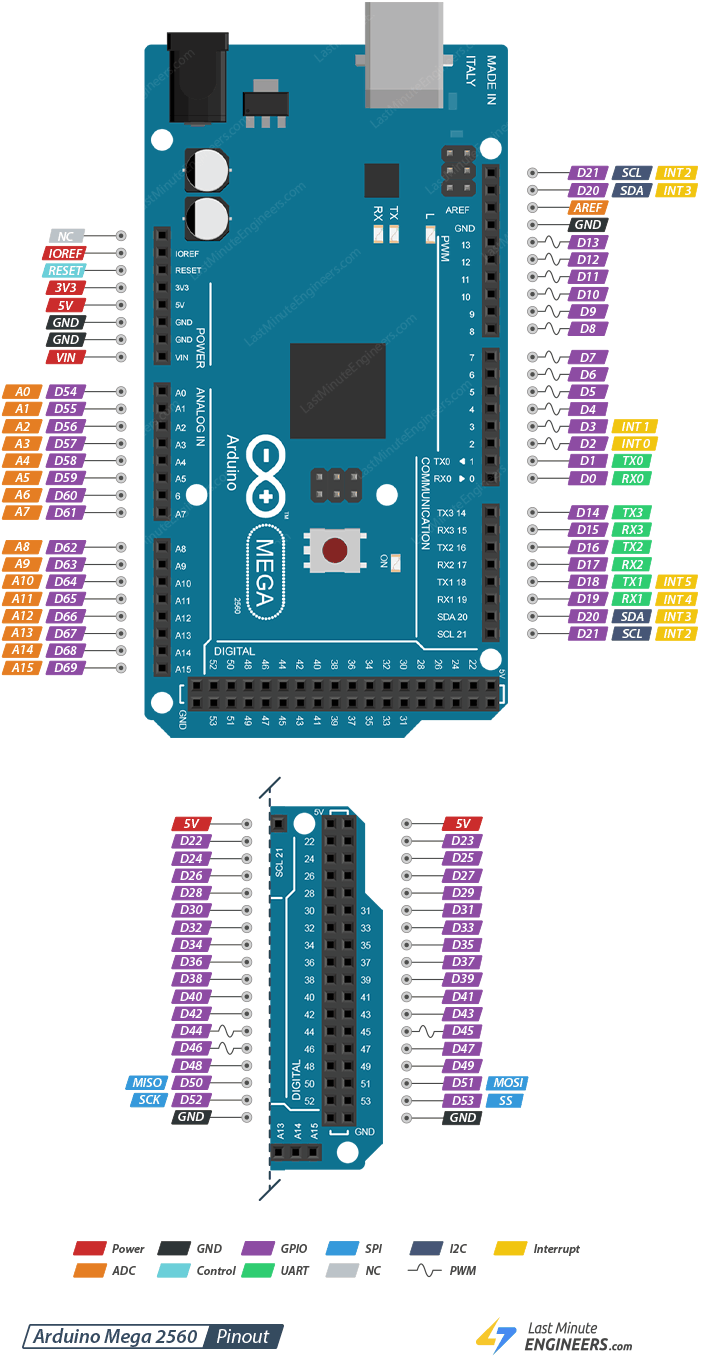
\includegraphics[width=0.75\textwidth]{images/pinout_arduino_mega.png} % Ganti dengan nama file gambar Anda
	\caption{Diagram pemetaan pin (\textit{pinout}) Arduino Mega 2560 (\href{https://lastminuteengineers.com/arduino-mega-pinout/}{Sumber: Last Minute Engineers}).}
	\label{fig:pinout_mega}
\end{figure}

% \subsection{Hubungan Konsep Mikrokontroler dengan Eksplorasi Komponen}
% Pemahaman konseptual mikrokontroler ini menjadi fondasi langsung untuk menganalisis komponen-komponen pada bagian selanjutnya:
% \begin{itemize}
%     \item Konsep **ADC** digunakan untuk menginterpretasikan pembacaan parameter kualitas udara dari sensor MQ-135 dan MQ-2.
%     \item Konsep **GPIO Digital** digunakan untuk membaca luaran biner dari sensor pergerakan HC-SR501 dan sensor jarak FC-51, serta mengendalikan logika aktivasi pada Modul Relay JQC-3FF-S-Z.
%     \item Konsep **PWM dan Timer** digunakan untuk membentuk pewaktuan presisi penentuan sudut pada Servo SG90 serta pengaturan kecepatan putar Motor DC 6V.
% \end{itemize}

\newpage

\section{Prinsip Kerja Setiap Komponen}
\label{sec:prinsip-komponen}

Bagian ini merupakan fokus utama FGD. Setiap komponen dibahas secara mandiri
agar pembaca memahami cara kerja, karakteristik sinyal, kebutuhan antarmuka,
dan batasan komponen sebelum melihat penerapannya dalam proyek.

\subsection{Cara Menggunakan Template Komponen}
Setiap komponen ditempatkan pada file terpisah di direktori
\texttt{sections/components/}. Gunakan struktur yang sama untuk setiap
komponen agar hasil eksplorasi dapat dibandingkan secara sistematis. Isi
bagian yang tidak relevan dengan \textit{Tidak berlaku} dan tambahkan
subsubsection khusus hanya jika memang diperlukan oleh karakteristik komponen.

% =====================================================================
% TEMPLATE ELABORASI SATU KOMPONEN
% Salin file ini menjadi komponen_NAMA.tex, lalu ganti placeholder.
% Jangan meng-input file template ini secara langsung ke bab.
% =====================================================================

\subsection{Komponen 1}
\label{subsec:komponen-01}

% ---------------------------------------------------------------------
\subsubsection{Identitas dan Fungsi}
Jelaskan nama komponen, produsen/model, kategori komponen (sensor, aktuator,
modul, atau komponen pendukung), fungsi utama, serta alasan komponen dipilih
untuk dieksplorasi.

\begin{table}[H]
\centering
\caption{Identitas komponen}
\begin{tabularx}{\textwidth}{@{}lX@{}}
\toprule
Parameter & Keterangan \\
\midrule
Nama komponen & \dots \\
Model/part number & \dots \\
Jenis & Sensor/Aktuator/Modul/Komponen pendukung \\
Fungsi utama & \dots \\
Sumber dokumentasi & \dots \\
\bottomrule
\end{tabularx}
\end{table}

% ---------------------------------------------------------------------
\subsubsection{Prinsip Kerja}
Jelaskan fenomena fisika atau elektronika yang membuat komponen memberikan
respons tertentu. Susun penjelasan dari kondisi masukan, proses internal,
hingga keluaran. Jika relevan, sertakan diagram, kurva karakteristik, atau
persamaan matematis.

% Contoh format persamaan:
% \begin{equation}
%   y = f(x)
%   \label{eq:komponen-nama}
% \end{equation}

\subsubsection{Alur Kerja Internal}
Uraikan alur \textbf{input \textrightarrow proses \textrightarrow output}.
Untuk sensor, jelaskan perubahan besaran fisik menjadi sinyal listrik.
Untuk aktuator, jelaskan perubahan sinyal listrik menjadi aksi fisik.
Jika komponen berupa modul digital, jelaskan proses pengolahan dan komunikasi
data secara konseptual.

% ---------------------------------------------------------------------
\subsubsection{Besaran yang Diukur atau Dikendalikan}
Jelaskan besaran utama, satuan, rentang pengukuran atau kendali, resolusi,
sensitivitas, akurasi, serta parameter lain yang relevan.

\begin{table}[H]
\centering
\caption{Karakteristik besaran komponen}
\begin{tabularx}{\textwidth}{@{}lXX@{}}
\toprule
Parameter & Nilai & Keterangan \\
\midrule
Besaran utama & \dots & \dots \\
Rentang & \dots & \dots \\
Resolusi & \dots & \dots \\
Akurasi/sensitivitas & \dots & \dots \\
\bottomrule
\end{tabularx}
\end{table}

% ---------------------------------------------------------------------
\subsubsection{Karakteristik Sinyal}
Identifikasi jenis sinyal dan jelaskan bentuk serta karakteristiknya. Bahas
apakah sinyal bersifat analog, digital, PWM, UART, I\textsuperscript{2}C,
SPI, atau protokol lain. Jelaskan level logika, rentang tegangan, frekuensi,
kecepatan data, resolusi ADC/DAC, atau parameter lain yang diperlukan.

\begin{table}[H]
\centering
\caption{Karakteristik sinyal}
\begin{tabularx}{\textwidth}{@{}lXX@{}}
\toprule
Aspek & Nilai & Keterangan \\
\midrule
Jenis sinyal & \dots & \dots \\
Level logika & \dots & \dots \\
Rentang tegangan & \dots & \dots \\
Frekuensi/baud rate & \dots & \dots \\
\bottomrule
\end{tabularx}
\end{table}

% ---------------------------------------------------------------------
\subsubsection{Pin, Catu Daya, dan Antarmuka}
Jelaskan fungsi setiap pin dan kebutuhan catu daya. Jika terdapat lebih dari
satu mode antarmuka, jelaskan perbedaannya dan alasan pemilihannya.

\begin{table}[H]
\centering
\caption{Pin dan antarmuka komponen}
\begin{tabularx}{\textwidth}{@{}lXX@{}}
\toprule
Pin/Antarmuka & Fungsi & Keterangan \\
\midrule
VCC/VIN & Catu daya & \dots \\
GND & Referensi & \dots \\
OUT/SDA/SCL/dll. & Sinyal & \dots \\
\bottomrule
\end{tabularx}
\end{table}

\subsubsection{Kebutuhan Catu Daya}
Jelaskan tegangan kerja, konsumsi arus, kondisi minimum/maksimum, kebutuhan
regulator, decoupling, serta kompatibilitas level tegangan dengan
mikrokontroler.

% ---------------------------------------------------------------------
\subsubsection{Spesifikasi Penting dari Datasheet}
Ambil hanya parameter yang relevan terhadap pemakaian komponen. Jangan sekadar
menyalin seluruh tabel datasheet; jelaskan arti setiap parameter dan mengapa
parameter tersebut penting untuk eksperimen.

\begin{table}[H]
\centering
\caption{Spesifikasi penting komponen}
\begin{tabular}{@{}lcc@{}}
\toprule
Parameter & Nilai & Satuan \\
\midrule
Tegangan kerja & \dots & \si{\volt} \\
Rentang ukur/keluaran & \dots & \dots \\
Resolusi/akurasi & \dots & \dots \\
Waktu respons & \dots & \si{\milli\second} \\
Arus konsumsi & \dots & \si{\milli\ampere} \\
\bottomrule
\end{tabular}
\end{table}

Sumber utama parameter: \cite{datasheet}.

% ---------------------------------------------------------------------
\subsubsection{Hubungan dengan Mikrokontroler}
Jelaskan fitur mikrokontroler yang digunakan, misalnya GPIO, ADC, timer,
interrupt, PWM, UART, I\textsuperscript{2}C, atau SPI. Kaitkan kebutuhan
tersebut dengan karakteristik sinyal komponen dan konsep pada Bagian B.
Referensi mikrokontroler dapat mengacu pada~\cite{mcu}.

\begin{table}[H]
\centering
\caption{Pemetaan komponen ke mikrokontroler}
\begin{tabularx}{\textwidth}{@{}lXX@{}}
\toprule
Kebutuhan komponen & Fitur MCU & Alasan pemilihan \\
\midrule
Input/output & \dots & \dots \\
Antarmuka komunikasi & \dots & \dots \\
Pemrosesan sinyal & \dots & \dots \\
\bottomrule
\end{tabularx}
\end{table}

% ---------------------------------------------------------------------
\subsubsection{Rangkaian Antarmuka}
Tampilkan skema koneksi komponen dengan mikrokontroler. Jelaskan aliran
sinyal dan fungsi setiap komponen eksternal. Jika ada resistor, kapasitor,
transistor, regulator, atau level shifter, sertakan dasar pemilihannya.

\begin{figure}[H]
\centering
% Ganti dengan gambar rangkaian aktual, misalnya:
% \includegraphics[width=0.85\textwidth]{images/rangkaian-nama-komponen.png}
\fbox{\parbox[c][4cm][c]{0.85\textwidth}{\centering Tempatkan skema rangkaian di sini}}
\caption{Rangkaian antarmuka Komponen 1 dengan mikrokontroler}
\label{fig:rangkaian-komponen-01}
\end{figure}

\subsubsection{Perhitungan dan Justifikasi Rangkaian}
Tunjukkan perhitungan yang diperlukan untuk menentukan nilai komponen
pendukung atau mengubah besaran sinyal. Jelaskan asumsi yang digunakan dan
bandingkan hasil perhitungan dengan batas datasheet.

% ---------------------------------------------------------------------
\subsubsection{Contoh Penggunaan Sederhana}
Buat eksperimen kecil yang hanya bertujuan memahami komponen. Jelaskan
input, prosedur, output yang diharapkan, dan indikator bahwa komponen bekerja
sesuai prinsipnya. Eksperimen ini harus dapat berdiri sendiri sebelum masuk
ke proyek utama.

\subsubsection{Program atau Algoritma Dasar}
Tampilkan bagian kode minimum yang diperlukan untuk membaca atau mengendalikan
komponen. Jelaskan fungsi bagian penting kode, bukan hanya menampilkan kode.

\begin{lstlisting}[caption={Contoh program dasar komponen}]
// Tulis kode minimum untuk menguji komponen di sini.
\end{lstlisting}

% ---------------------------------------------------------------------
\subsubsection{Hasil Eksplorasi}
Dokumentasikan hasil pengamatan, nilai pembacaan, respons komponen, foto,
grafik, atau bukti lain. Bedakan antara hasil yang diharapkan berdasarkan
teori dan hasil aktual.

\begin{table}[H]
\centering
\caption{Contoh format hasil eksplorasi}
\begin{tabularx}{\textwidth}{@{}lXX@{}}
\toprule
Kondisi/Input & Hasil Teoretis & Hasil Pengamatan \\
\midrule
Kondisi 1 & \dots & \dots \\
Kondisi 2 & \dots & \dots \\
Kondisi 3 & \dots & \dots \\
\bottomrule
\end{tabularx}
\end{table}

% ---------------------------------------------------------------------
\subsubsection{Analisis dan Interpretasi}
Hubungkan hasil eksplorasi dengan prinsip kerja dan spesifikasi datasheet.
Jelaskan apakah hasil sesuai teori, penyebab perbedaan, serta implikasinya
terhadap penggunaan komponen pada proyek.

\subsubsection{Keterbatasan dan Sumber Kesalahan}
Bahas noise, toleransi komponen, kesalahan pembacaan, kalibrasi, temperatur,
kondisi lingkungan, keterbatasan library, keterbatasan catu daya, batas
komunikasi, atau faktor lain yang dapat memengaruhi hasil.

\subsubsection{Kesimpulan Pemahaman Komponen}
Tuliskan secara ringkas apa yang dapat disimpulkan mengenai prinsip kerja,
karakteristik sinyal, kebutuhan mikrokontroler, dan kondisi penggunaan
komponen. Tekankan bukti yang menunjukkan bahwa prinsip kerja telah dipahami.

% =====================================================================
% TEMPLATE ELABORASI SATU KOMPONEN
% Salin file ini menjadi komponen_NAMA.tex, lalu ganti placeholder.
% Jangan meng-input file template ini secara langsung ke bab.
% =====================================================================

\subsection{Komponen 2}
\label{subsec:komponen-02}

% ---------------------------------------------------------------------
\subsubsection{Identitas dan Fungsi}
Jelaskan nama komponen, produsen/model, kategori komponen (sensor, aktuator,
modul, atau komponen pendukung), fungsi utama, serta alasan komponen dipilih
untuk dieksplorasi.

\begin{table}[H]
\centering
\caption{Identitas komponen}
\begin{tabularx}{\textwidth}{@{}lX@{}}
\toprule
Parameter & Keterangan \\
\midrule
Nama komponen & \dots \\
Model/part number & \dots \\
Jenis & Sensor/Aktuator/Modul/Komponen pendukung \\
Fungsi utama & \dots \\
Sumber dokumentasi & \dots \\
\bottomrule
\end{tabularx}
\end{table}

% ---------------------------------------------------------------------
\subsubsection{Prinsip Kerja}
Jelaskan fenomena fisika atau elektronika yang membuat komponen memberikan
respons tertentu. Susun penjelasan dari kondisi masukan, proses internal,
hingga keluaran. Jika relevan, sertakan diagram, kurva karakteristik, atau
persamaan matematis.

% Contoh format persamaan:
% \begin{equation}
%   y = f(x)
%   \label{eq:komponen-nama}
% \end{equation}

\subsubsection{Alur Kerja Internal}
Uraikan alur \textbf{input \textrightarrow proses \textrightarrow output}.
Untuk sensor, jelaskan perubahan besaran fisik menjadi sinyal listrik.
Untuk aktuator, jelaskan perubahan sinyal listrik menjadi aksi fisik.
Jika komponen berupa modul digital, jelaskan proses pengolahan dan komunikasi
data secara konseptual.

% ---------------------------------------------------------------------
\subsubsection{Besaran yang Diukur atau Dikendalikan}
Jelaskan besaran utama, satuan, rentang pengukuran atau kendali, resolusi,
sensitivitas, akurasi, serta parameter lain yang relevan.

\begin{table}[H]
\centering
\caption{Karakteristik besaran komponen}
\begin{tabularx}{\textwidth}{@{}lXX@{}}
\toprule
Parameter & Nilai & Keterangan \\
\midrule
Besaran utama & \dots & \dots \\
Rentang & \dots & \dots \\
Resolusi & \dots & \dots \\
Akurasi/sensitivitas & \dots & \dots \\
\bottomrule
\end{tabularx}
\end{table}

% ---------------------------------------------------------------------
\subsubsection{Karakteristik Sinyal}
Identifikasi jenis sinyal dan jelaskan bentuk serta karakteristiknya. Bahas
apakah sinyal bersifat analog, digital, PWM, UART, I\textsuperscript{2}C,
SPI, atau protokol lain. Jelaskan level logika, rentang tegangan, frekuensi,
kecepatan data, resolusi ADC/DAC, atau parameter lain yang diperlukan.

\begin{table}[H]
\centering
\caption{Karakteristik sinyal}
\begin{tabularx}{\textwidth}{@{}lXX@{}}
\toprule
Aspek & Nilai & Keterangan \\
\midrule
Jenis sinyal & \dots & \dots \\
Level logika & \dots & \dots \\
Rentang tegangan & \dots & \dots \\
Frekuensi/baud rate & \dots & \dots \\
\bottomrule
\end{tabularx}
\end{table}

% ---------------------------------------------------------------------
\subsubsection{Pin, Catu Daya, dan Antarmuka}
Jelaskan fungsi setiap pin dan kebutuhan catu daya. Jika terdapat lebih dari
satu mode antarmuka, jelaskan perbedaannya dan alasan pemilihannya.

\begin{table}[H]
\centering
\caption{Pin dan antarmuka komponen}
\begin{tabularx}{\textwidth}{@{}lXX@{}}
\toprule
Pin/Antarmuka & Fungsi & Keterangan \\
\midrule
VCC/VIN & Catu daya & \dots \\
GND & Referensi & \dots \\
OUT/SDA/SCL/dll. & Sinyal & \dots \\
\bottomrule
\end{tabularx}
\end{table}

\subsubsection{Kebutuhan Catu Daya}
Jelaskan tegangan kerja, konsumsi arus, kondisi minimum/maksimum, kebutuhan
regulator, decoupling, serta kompatibilitas level tegangan dengan
mikrokontroler.

% ---------------------------------------------------------------------
\subsubsection{Spesifikasi Penting dari Datasheet}
Ambil hanya parameter yang relevan terhadap pemakaian komponen. Jangan sekadar
menyalin seluruh tabel datasheet; jelaskan arti setiap parameter dan mengapa
parameter tersebut penting untuk eksperimen.

\begin{table}[H]
\centering
\caption{Spesifikasi penting komponen}
\begin{tabular}{@{}lcc@{}}
\toprule
Parameter & Nilai & Satuan \\
\midrule
Tegangan kerja & \dots & \si{\volt} \\
Rentang ukur/keluaran & \dots & \dots \\
Resolusi/akurasi & \dots & \dots \\
Waktu respons & \dots & \si{\milli\second} \\
Arus konsumsi & \dots & \si{\milli\ampere} \\
\bottomrule
\end{tabular}
\end{table}

Sumber utama parameter: \cite{datasheet}.

% ---------------------------------------------------------------------
\subsubsection{Hubungan dengan Mikrokontroler}
Jelaskan fitur mikrokontroler yang digunakan, misalnya GPIO, ADC, timer,
interrupt, PWM, UART, I\textsuperscript{2}C, atau SPI. Kaitkan kebutuhan
tersebut dengan karakteristik sinyal komponen dan konsep pada Bagian B.
Referensi mikrokontroler dapat mengacu pada~\cite{mcu}.

\begin{table}[H]
\centering
\caption{Pemetaan komponen ke mikrokontroler}
\begin{tabularx}{\textwidth}{@{}lXX@{}}
\toprule
Kebutuhan komponen & Fitur MCU & Alasan pemilihan \\
\midrule
Input/output & \dots & \dots \\
Antarmuka komunikasi & \dots & \dots \\
Pemrosesan sinyal & \dots & \dots \\
\bottomrule
\end{tabularx}
\end{table}

% ---------------------------------------------------------------------
\subsubsection{Rangkaian Antarmuka}
Tampilkan skema koneksi komponen dengan mikrokontroler. Jelaskan aliran
sinyal dan fungsi setiap komponen eksternal. Jika ada resistor, kapasitor,
transistor, regulator, atau level shifter, sertakan dasar pemilihannya.

\begin{figure}[H]
\centering
% Ganti dengan gambar rangkaian aktual, misalnya:
% \includegraphics[width=0.85\textwidth]{images/rangkaian-nama-komponen.png}
\fbox{\parbox[c][4cm][c]{0.85\textwidth}{\centering Tempatkan skema rangkaian di sini}}
\caption{Rangkaian antarmuka Komponen 2 dengan mikrokontroler}
\label{fig:rangkaian-komponen-02}
\end{figure}

\subsubsection{Perhitungan dan Justifikasi Rangkaian}
Tunjukkan perhitungan yang diperlukan untuk menentukan nilai komponen
pendukung atau mengubah besaran sinyal. Jelaskan asumsi yang digunakan dan
bandingkan hasil perhitungan dengan batas datasheet.

% ---------------------------------------------------------------------
\subsubsection{Contoh Penggunaan Sederhana}
Buat eksperimen kecil yang hanya bertujuan memahami komponen. Jelaskan
input, prosedur, output yang diharapkan, dan indikator bahwa komponen bekerja
sesuai prinsipnya. Eksperimen ini harus dapat berdiri sendiri sebelum masuk
ke proyek utama.

\subsubsection{Program atau Algoritma Dasar}
Tampilkan bagian kode minimum yang diperlukan untuk membaca atau mengendalikan
komponen. Jelaskan fungsi bagian penting kode, bukan hanya menampilkan kode.

\begin{lstlisting}[caption={Contoh program dasar komponen}]
// Tulis kode minimum untuk menguji komponen di sini.
\end{lstlisting}

% ---------------------------------------------------------------------
\subsubsection{Hasil Eksplorasi}
Dokumentasikan hasil pengamatan, nilai pembacaan, respons komponen, foto,
grafik, atau bukti lain. Bedakan antara hasil yang diharapkan berdasarkan
teori dan hasil aktual.

\begin{table}[H]
\centering
\caption{Contoh format hasil eksplorasi}
\begin{tabularx}{\textwidth}{@{}lXX@{}}
\toprule
Kondisi/Input & Hasil Teoretis & Hasil Pengamatan \\
\midrule
Kondisi 1 & \dots & \dots \\
Kondisi 2 & \dots & \dots \\
Kondisi 3 & \dots & \dots \\
\bottomrule
\end{tabularx}
\end{table}

% ---------------------------------------------------------------------
\subsubsection{Analisis dan Interpretasi}
Hubungkan hasil eksplorasi dengan prinsip kerja dan spesifikasi datasheet.
Jelaskan apakah hasil sesuai teori, penyebab perbedaan, serta implikasinya
terhadap penggunaan komponen pada proyek.

\subsubsection{Keterbatasan dan Sumber Kesalahan}
Bahas noise, toleransi komponen, kesalahan pembacaan, kalibrasi, temperatur,
kondisi lingkungan, keterbatasan library, keterbatasan catu daya, batas
komunikasi, atau faktor lain yang dapat memengaruhi hasil.

\subsubsection{Kesimpulan Pemahaman Komponen}
Tuliskan secara ringkas apa yang dapat disimpulkan mengenai prinsip kerja,
karakteristik sinyal, kebutuhan mikrokontroler, dan kondisi penggunaan
komponen. Tekankan bukti yang menunjukkan bahwa prinsip kerja telah dipahami.

% =====================================================================
% TEMPLATE ELABORASI SATU KOMPONEN
% Salin file ini menjadi komponen_NAMA.tex, lalu ganti placeholder.
% Jangan meng-input file template ini secara langsung ke bab.
% =====================================================================

\subsection{Komponen 3}
\label{subsec:komponen-03}

% ---------------------------------------------------------------------
\subsubsection{Identitas dan Fungsi}
Jelaskan nama komponen, produsen/model, kategori komponen (sensor, aktuator,
modul, atau komponen pendukung), fungsi utama, serta alasan komponen dipilih
untuk dieksplorasi.

\begin{table}[H]
\centering
\caption{Identitas komponen}
\begin{tabularx}{\textwidth}{@{}lX@{}}
\toprule
Parameter & Keterangan \\
\midrule
Nama komponen & \dots \\
Model/part number & \dots \\
Jenis & Sensor/Aktuator/Modul/Komponen pendukung \\
Fungsi utama & \dots \\
Sumber dokumentasi & \dots \\
\bottomrule
\end{tabularx}
\end{table}

% ---------------------------------------------------------------------
\subsubsection{Prinsip Kerja}
Jelaskan fenomena fisika atau elektronika yang membuat komponen memberikan
respons tertentu. Susun penjelasan dari kondisi masukan, proses internal,
hingga keluaran. Jika relevan, sertakan diagram, kurva karakteristik, atau
persamaan matematis.

% Contoh format persamaan:
% \begin{equation}
%   y = f(x)
%   \label{eq:komponen-nama}
% \end{equation}

\subsubsection{Alur Kerja Internal}
Uraikan alur \textbf{input \textrightarrow proses \textrightarrow output}.
Untuk sensor, jelaskan perubahan besaran fisik menjadi sinyal listrik.
Untuk aktuator, jelaskan perubahan sinyal listrik menjadi aksi fisik.
Jika komponen berupa modul digital, jelaskan proses pengolahan dan komunikasi
data secara konseptual.

% ---------------------------------------------------------------------
\subsubsection{Besaran yang Diukur atau Dikendalikan}
Jelaskan besaran utama, satuan, rentang pengukuran atau kendali, resolusi,
sensitivitas, akurasi, serta parameter lain yang relevan.

\begin{table}[H]
\centering
\caption{Karakteristik besaran komponen}
\begin{tabularx}{\textwidth}{@{}lXX@{}}
\toprule
Parameter & Nilai & Keterangan \\
\midrule
Besaran utama & \dots & \dots \\
Rentang & \dots & \dots \\
Resolusi & \dots & \dots \\
Akurasi/sensitivitas & \dots & \dots \\
\bottomrule
\end{tabularx}
\end{table}

% ---------------------------------------------------------------------
\subsubsection{Karakteristik Sinyal}
Identifikasi jenis sinyal dan jelaskan bentuk serta karakteristiknya. Bahas
apakah sinyal bersifat analog, digital, PWM, UART, I\textsuperscript{2}C,
SPI, atau protokol lain. Jelaskan level logika, rentang tegangan, frekuensi,
kecepatan data, resolusi ADC/DAC, atau parameter lain yang diperlukan.

\begin{table}[H]
\centering
\caption{Karakteristik sinyal}
\begin{tabularx}{\textwidth}{@{}lXX@{}}
\toprule
Aspek & Nilai & Keterangan \\
\midrule
Jenis sinyal & \dots & \dots \\
Level logika & \dots & \dots \\
Rentang tegangan & \dots & \dots \\
Frekuensi/baud rate & \dots & \dots \\
\bottomrule
\end{tabularx}
\end{table}

% ---------------------------------------------------------------------
\subsubsection{Pin, Catu Daya, dan Antarmuka}
Jelaskan fungsi setiap pin dan kebutuhan catu daya. Jika terdapat lebih dari
satu mode antarmuka, jelaskan perbedaannya dan alasan pemilihannya.

\begin{table}[H]
\centering
\caption{Pin dan antarmuka komponen}
\begin{tabularx}{\textwidth}{@{}lXX@{}}
\toprule
Pin/Antarmuka & Fungsi & Keterangan \\
\midrule
VCC/VIN & Catu daya & \dots \\
GND & Referensi & \dots \\
OUT/SDA/SCL/dll. & Sinyal & \dots \\
\bottomrule
\end{tabularx}
\end{table}

\subsubsection{Kebutuhan Catu Daya}
Jelaskan tegangan kerja, konsumsi arus, kondisi minimum/maksimum, kebutuhan
regulator, decoupling, serta kompatibilitas level tegangan dengan
mikrokontroler.

% ---------------------------------------------------------------------
\subsubsection{Spesifikasi Penting dari Datasheet}
Ambil hanya parameter yang relevan terhadap pemakaian komponen. Jangan sekadar
menyalin seluruh tabel datasheet; jelaskan arti setiap parameter dan mengapa
parameter tersebut penting untuk eksperimen.

\begin{table}[H]
\centering
\caption{Spesifikasi penting komponen}
\begin{tabular}{@{}lcc@{}}
\toprule
Parameter & Nilai & Satuan \\
\midrule
Tegangan kerja & \dots & \si{\volt} \\
Rentang ukur/keluaran & \dots & \dots \\
Resolusi/akurasi & \dots & \dots \\
Waktu respons & \dots & \si{\milli\second} \\
Arus konsumsi & \dots & \si{\milli\ampere} \\
\bottomrule
\end{tabular}
\end{table}

Sumber utama parameter: \cite{datasheet}.

% ---------------------------------------------------------------------
\subsubsection{Hubungan dengan Mikrokontroler}
Jelaskan fitur mikrokontroler yang digunakan, misalnya GPIO, ADC, timer,
interrupt, PWM, UART, I\textsuperscript{2}C, atau SPI. Kaitkan kebutuhan
tersebut dengan karakteristik sinyal komponen dan konsep pada Bagian B.
Referensi mikrokontroler dapat mengacu pada~\cite{mcu}.

\begin{table}[H]
\centering
\caption{Pemetaan komponen ke mikrokontroler}
\begin{tabularx}{\textwidth}{@{}lXX@{}}
\toprule
Kebutuhan komponen & Fitur MCU & Alasan pemilihan \\
\midrule
Input/output & \dots & \dots \\
Antarmuka komunikasi & \dots & \dots \\
Pemrosesan sinyal & \dots & \dots \\
\bottomrule
\end{tabularx}
\end{table}

% ---------------------------------------------------------------------
\subsubsection{Rangkaian Antarmuka}
Tampilkan skema koneksi komponen dengan mikrokontroler. Jelaskan aliran
sinyal dan fungsi setiap komponen eksternal. Jika ada resistor, kapasitor,
transistor, regulator, atau level shifter, sertakan dasar pemilihannya.

\begin{figure}[H]
\centering
% Ganti dengan gambar rangkaian aktual, misalnya:
% \includegraphics[width=0.85\textwidth]{images/rangkaian-nama-komponen.png}
\fbox{\parbox[c][4cm][c]{0.85\textwidth}{\centering Tempatkan skema rangkaian di sini}}
\caption{Rangkaian antarmuka Komponen 3 dengan mikrokontroler}
\label{fig:rangkaian-komponen-03}
\end{figure}

\subsubsection{Perhitungan dan Justifikasi Rangkaian}
Tunjukkan perhitungan yang diperlukan untuk menentukan nilai komponen
pendukung atau mengubah besaran sinyal. Jelaskan asumsi yang digunakan dan
bandingkan hasil perhitungan dengan batas datasheet.

% ---------------------------------------------------------------------
\subsubsection{Contoh Penggunaan Sederhana}
Buat eksperimen kecil yang hanya bertujuan memahami komponen. Jelaskan
input, prosedur, output yang diharapkan, dan indikator bahwa komponen bekerja
sesuai prinsipnya. Eksperimen ini harus dapat berdiri sendiri sebelum masuk
ke proyek utama.

\subsubsection{Program atau Algoritma Dasar}
Tampilkan bagian kode minimum yang diperlukan untuk membaca atau mengendalikan
komponen. Jelaskan fungsi bagian penting kode, bukan hanya menampilkan kode.

\begin{lstlisting}[caption={Contoh program dasar komponen}]
// Tulis kode minimum untuk menguji komponen di sini.
\end{lstlisting}

% ---------------------------------------------------------------------
\subsubsection{Hasil Eksplorasi}
Dokumentasikan hasil pengamatan, nilai pembacaan, respons komponen, foto,
grafik, atau bukti lain. Bedakan antara hasil yang diharapkan berdasarkan
teori dan hasil aktual.

\begin{table}[H]
\centering
\caption{Contoh format hasil eksplorasi}
\begin{tabularx}{\textwidth}{@{}lXX@{}}
\toprule
Kondisi/Input & Hasil Teoretis & Hasil Pengamatan \\
\midrule
Kondisi 1 & \dots & \dots \\
Kondisi 2 & \dots & \dots \\
Kondisi 3 & \dots & \dots \\
\bottomrule
\end{tabularx}
\end{table}

% ---------------------------------------------------------------------
\subsubsection{Analisis dan Interpretasi}
Hubungkan hasil eksplorasi dengan prinsip kerja dan spesifikasi datasheet.
Jelaskan apakah hasil sesuai teori, penyebab perbedaan, serta implikasinya
terhadap penggunaan komponen pada proyek.

\subsubsection{Keterbatasan dan Sumber Kesalahan}
Bahas noise, toleransi komponen, kesalahan pembacaan, kalibrasi, temperatur,
kondisi lingkungan, keterbatasan library, keterbatasan catu daya, batas
komunikasi, atau faktor lain yang dapat memengaruhi hasil.

\subsubsection{Kesimpulan Pemahaman Komponen}
Tuliskan secara ringkas apa yang dapat disimpulkan mengenai prinsip kerja,
karakteristik sinyal, kebutuhan mikrokontroler, dan kondisi penggunaan
komponen. Tekankan bukti yang menunjukkan bahwa prinsip kerja telah dipahami.


\subsection{Perbandingan Antar-Komponen}
Setelah setiap komponen dibahas secara mandiri, bandingkan karakteristik yang
paling penting untuk menunjukkan alasan pemilihan komponen dan hubungan
masing-masing komponen dengan mikrokontroler.
\begin{table}[H]
\centering
\caption{Perbandingan karakteristik komponen}
\begin{tabularx}{\textwidth}{@{}lXXX@{}}
\toprule
Aspek & Komponen 1 & Komponen 2 & Komponen 3 \\
\midrule
Besaran utama & \dots & \dots & \dots \\
Jenis sinyal & \dots & \dots & \dots \\
Antarmuka MCU & \dots & \dots & \dots \\
Kebutuhan daya & \dots & \dots & \dots \\
Keterbatasan utama & \dots & \dots & \dots \\
\bottomrule
\end{tabularx}
\end{table}

\subsection{Komponen Pendukung}
Jelaskan komponen pendukung yang diperlukan agar komponen utama bekerja
sesuai spesifikasi, misalnya resistor pull-up/pull-down, kapasitor decoupling,
dioda proteksi, transistor driver, regulator, atau level shifter. Hubungkan
setiap komponen pendukung dengan kebutuhan komponen utama yang telah dibahas.

\newpage

\section{Proyek -- Sistem Deteksi Gas \& Penanganan Darurat Otomatis}
\label{sec:proyek-eksperimen}

Proyek ini dirancang untuk menguji integrasi multikomponen berbasis interupsi eksternal dan kontrol non-pemblokiran (\textit{non-blocking}) pada mikrokontroler Arduino Mega 2560. Sistem menggabungkan logika operasional harian (akses pintu otomatis berbasis gerakan) dan logika penanganan darurat prioritas tinggi (mitigasi kebocoran gas).
\subsection{Desain Sistem}
\label{subsec:desain_sistem}

Sistem keselamatan ini dirancang menggunakan arsitektur dual-mode berbasis prioritas pemrosesan: \textbf{Mode Reguler} (manajemen akses pintu otomatis berbasis deteksi gerakan) dan \textbf{Mode Darurat} (mitigasi kebocoran gas berbasis interupsi eksternal \textit{hardware}).

Interkoneksi fisik dan alokasi pin antarmuka mikrokontroler Arduino Mega 2560 disajikan secara terisolasi pada Gambar~\ref{fig:blok_simpel}.

\begin{figure}[htbp]
	\centering
	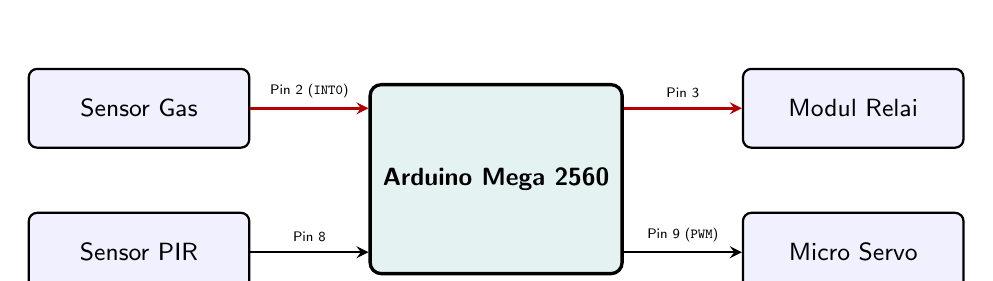
\begin{tikzpicture}[
			node distance=1.5cm and 1.5cm,
			blok/.style={draw, rectangle, rounded corners=3pt, minimum width=2.8cm, minimum height=1.0cm, align=center, font=\sffamily\small, fill=blue!6, line width=0.8pt},
			mcu/.style={draw, rectangle, rounded corners=4pt, minimum width=3.2cm, minimum height=2.4cm, align=center, font=\sffamily\small, fill=teal!10, line width=1.2pt},
			panah/.style={->, >=stealth, thick, line width=0.9pt}
		]
		% Node Input (Kiri)
		\node[blok] (gas) {Sensor Gas};
		\node[blok, below=0.8cm of gas] (pir) {Sensor PIR};

		% Node MCU (Tengah)
		\node[mcu, right=1.5cm of gas, yshift=-0.9cm] (mcu) {\textbf{Arduino Mega 2560}};

		% Node Output (Kanan)
		\node[blok, right=1.5cm of mcu, yshift=0.9cm] (relay) {Modul Relai};
		\node[blok, below=0.8cm of relay] (servo) {Micro Servo};

		% Garis Penghubung Input ke MCU
		\draw[panah, color=red!70!black] (gas.east) -- node[above, font=\tiny\sffamily, color=black] {Pin 2 (\texttt{INT0})} (gas.east -| mcu.west);
		\draw[panah] (pir.east) -- node[above, font=\tiny\sffamily, color=black] {Pin 8} (pir.east -| mcu.west);

		% Garis Penghubung MCU ke Output
		\draw[panah, color=red!70!black] (mcu.east |- relay.west) -- node[above, font=\tiny\sffamily, color=black] {Pin 3} (relay.west);
		\draw[panah] (mcu.east |- servo.west) -- node[above, font=\tiny\sffamily, color=black] {Pin 9 (\texttt{PWM})} (servo.west);
	\end{tikzpicture}
	\caption{Diagram blok antarmuka periferal dan aktuator sistem.}
	\label{fig:blok_simpel}
\end{figure}

Alur eksekusi logika dipisahkan secara tegas berdasarkan status atmosferik lingkungan:

\begin{enumerate}
	\item \textbf{Alur Operasi Normal (PIR \& Pintu Otomatis):} Pada kondisi aman, mikrokontroler mengeksekusi \textit{polling} non-pemblokiran (\textit{non-blocking}) memanfaatkan pewaktu internal \texttt{millis()}. Jika sensor PIR mendeteksi gerakan (logika \texttt{HIGH}), \textit{servo motor} bergerak ke sudut $140^\circ$. Pintu akan dipertahankan terbuka selama penunda waktu (\textit{hold time}) minimal $1000\,\text{ms}$ sebelum ditutup kembali ke sudut $45^\circ$.
	\item \textbf{Alur Penanganan Darurat (Interupsi Kebocoran Gas):} Saat sensor gas mendeteksi kebocoran, keluaran digital berubah menjadi \texttt{LOW} (\textit{Active-LOW}) dan langsung memicu interupsi \texttt{INT0} pada pemicuan tepi turun (\textit{FALLING edge}). Rutin \textit{Interrupt Service Routine} (ISR) mengesampingkan eksekusi normal, mengaktifkan kipas pembuang udara melalui modul relai (Pin 3 \texttt{HIGH}), serta mematikan dan mengunci posisi pintu servo pada sudut $45^\circ$ hingga udara dinyatakan aman.
\end{enumerate}

Diagram alur (\textit{flowchart}) untuk kedua mode operasional disajikan secara bersandingan menggunakan \textit{subfigure} pada Gambar~\ref{fig:flowcharts_side_by_side}.

\begin{figure}[htbp]
	\centering
	% ------------------ SUBFIGURE 1: ALUR NORMAL (KIRI) ------------------
	\begin{subfigure}[t]{0.49\textwidth}
		\centering
		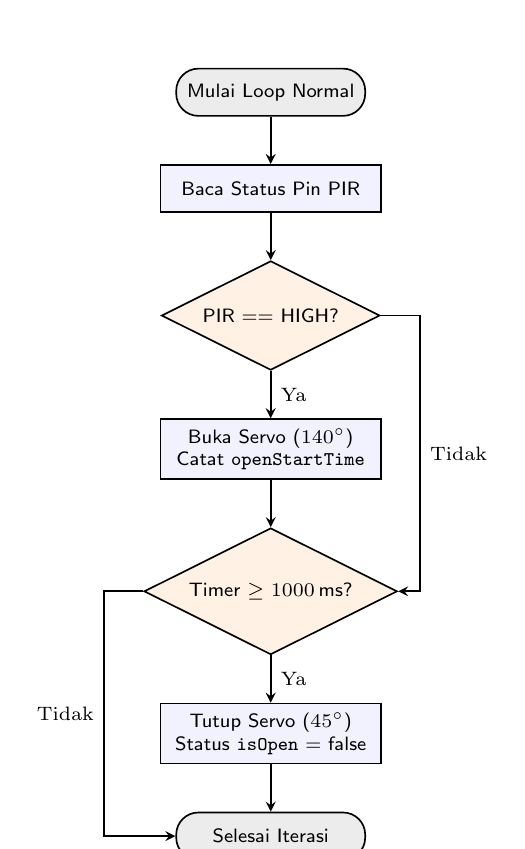
\begin{tikzpicture}[
				node distance=0.6cm,
				startend/.style={draw, rectangle, rounded corners=8pt, minimum width=2.4cm, minimum height=0.6cm, align=center, font=\sffamily\scriptsize, fill=gray!15, line width=0.6pt},
				proses/.style={draw, rectangle, minimum width=2.8cm, minimum height=0.6cm, align=center, font=\sffamily\scriptsize, fill=blue!5, line width=0.6pt},
				keputusan/.style={draw, diamond, aspect=2, minimum width=2.6cm, minimum height=0.7cm, align=center, font=\sffamily\scriptsize, fill=orange!10, line width=0.6pt},
				panah/.style={->, >=stealth, semithick}
			]
			\node[startend] (start) {Mulai Loop Normal};
			\node[proses, below=of start] (read) {Baca Status Pin PIR};
			\node[keputusan, below=of read] (cek_pir) {PIR == HIGH?};
			\node[proses, below=of cek_pir] (buka) {Buka Servo ($140^\circ$)\\Catat \texttt{openStartTime}};
			\node[keputusan, below=of buka] (cek_timer) {Timer $\ge 1000\,\text{ms}$?};
			\node[proses, below=of cek_timer] (tutup) {Tutup Servo ($45^\circ$)\\Status \texttt{isOpen} = false};
			\node[startend, below=of tutup] (end) {Selesai Iterasi};

			% Garis Alur Utama
			\draw[panah] (start) -- (read);
			\draw[panah] (read) -- (cek_pir);
			\draw[panah] (cek_pir) -- node[right, font=\scriptsize] {Ya} (buka);
			\draw[panah] (buka) -- (cek_timer);
			\draw[panah] (cek_timer) -- node[right, font=\scriptsize] {Ya} (tutup);
			\draw[panah] (tutup) -- (end);

			% Garis Bypass (Tidak)
			\draw[panah] (cek_pir.east) -- ++(0.5,0) |- node[near start, right, font=\scriptsize] {Tidak} (cek_timer.east);
			\draw[panah] (cek_timer.west) -- ++(-0.5,0) |- node[near start, left, font=\scriptsize] {Tidak} (end.west);
		\end{tikzpicture}
		\caption{Mode reguler (PIR \& Servo).}
		\label{fig:flowchart_normal_sub}
	\end{subfigure}
	\hfill
	% ------------------ SUBFIGURE 2: ALUR DARURAT (KANAN) ------------------
	\begin{subfigure}[t]{0.49\textwidth}
		\centering
		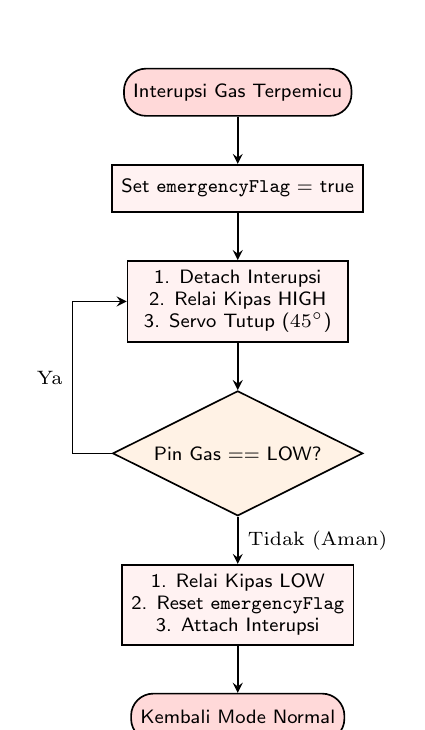
\begin{tikzpicture}[
				node distance=0.6cm,
				startend/.style={draw, rectangle, rounded corners=8pt, minimum width=2.4cm, minimum height=0.6cm, align=center, font=\sffamily\scriptsize, fill=red!15, line width=0.6pt},
				proses/.style={draw, rectangle, minimum width=2.8cm, minimum height=0.6cm, align=center, font=\sffamily\scriptsize, fill=red!5, line width=0.6pt},
				keputusan/.style={draw, diamond, aspect=2, minimum width=2.6cm, minimum height=0.7cm, align=center, font=\sffamily\scriptsize, fill=orange!10, line width=0.6pt},
				panah/.style={->, >=stealth, semithick}
			]
			\node[startend] (start) {Interupsi Gas Terpemicu};
			\node[proses, below=of start] (flag) {Set \texttt{emergencyFlag} = true};
			\node[proses, below=of flag] (action) {1. Detach Interupsi\\2. Relai Kipas HIGH\\3. Servo Tutup ($45^\circ$)};
			\node[keputusan, below=of action] (cek_gas) {Pin Gas == LOW?};
			\node[proses, below=of cek_gas] (clear) {1. Relai Kipas LOW\\2. Reset \texttt{emergencyFlag}\\3. Attach Interupsi};
			\node[startend, below=of clear] (end) {Kembali Mode Normal};

			% Garis Alur Utama
			\draw[panah] (start) -- (flag);
			\draw[panah] (flag) -- (action);
			\draw[panah] (action) -- (cek_gas);
			\draw[panah] (cek_gas) -- node[right, font=\scriptsize] {Tidak (Aman)} (clear);
			\draw[panah] (clear) -- (end);

			% Garis Loop Kondisi Masih Ada Gas (Ya)
			\draw[panah] (cek_gas.west) -- ++(-0.5,0) |- node[near start, left, font=\scriptsize] {Ya} (action.west);
		\end{tikzpicture}
		\caption{Mode darurat (Interupsi Gas).}
		\label{fig:flowchart_emergency_sub}
	\end{subfigure}
	\caption{Diagram alur logika eksekusi sistem: (a) Mode operasional harian berbasis PIR dan (b) Mode penanganan kebocoran gas berbasis interupsi.}
	\label{fig:flowcharts_side_by_side}
\end{figure}

\subsection{Rangkaian dan Koneksi}
Pemetaan koneksi fisik antara komponen antarmuka dan mikrokontroler Arduino Mega 2560 dirangkum pada Tabel~\ref{tab:koneksi_proyek}.

\begin{figure}[htbp]
	\centering
	% Ganti dengan file skematik rangkaian aktual atau tangkapan layar simulasi Wokwi
	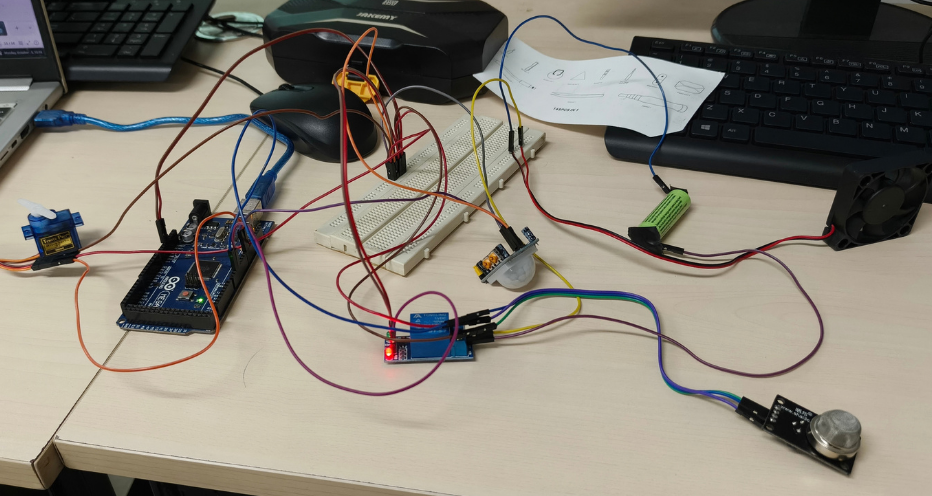
\includegraphics[width=0.70\textwidth]{images/rangkaian_proyek.png}
	% \fbox{\parbox[c][5cm][c]{0.70\textwidth}{\centering Tempatkan tangkapan layar simulasi Wokwi atau diagram skematik antarmuka Sensor MQ dengan Arduino Mega 2560 di sini}}
	\caption{Rangkaian Sistem Deteksi Gas \& Penanganan Darurat Otomatis.}
	\label{fig:rangkaian_sistem}
\end{figure}



\begin{table}[H]
	\centering
	\caption{Pemetaan antarmuka komponen ke Arduino Mega 2560}
	\label{tab:koneksi_proyek}
	\small
	\begin{tabularx}{\textwidth}{@{} p{3.2cm} p{3.8cm} X @{}}
		\toprule
		Komponen          & Pin MCU                       & Alasan Pemilihan \& Fungsi                                                             \\
		\midrule
		Sensor Gas (DOUT) & Pin Digital 2 (\texttt{INT0}) & Mendukung fitur interupsi eksternal hardware untuk deteksi kebocoran gas secara instan \\
		Sensor PIR (OUT)  & Pin Digital 8                 & Membaca logika keberadaan objek untuk aktuasi pintu otomatis                           \\
		Modul Relai (IN)  & Pin Digital 3                 & Sakelar daya beban induktif kipas eksternal                                            \\
		Servo Motor (PWM) & Pin Digital 9                 & Mengendalikan sudut bukaan engsel pintu otomatis ($45^\circ\text{--}140^\circ$)        \\
		\bottomrule
	\end{tabularx}
\end{table}

\subsection{Program Eksperimen}
Kode program diimplementasikan menggunakan arsitektur \textit{state machine} sederhana yang mengisolasi eksekusi mode reguler dan mode darurat melalui bendera interupsi \textit{volatile} (\texttt{emergencyFlag}).

\begin{lstlisting}[language=C++, caption={Kode program sistem deteksi gas dan penanganan darurat otomatis}, label={lst:proyek_code}]
#include <Servo.h>

const int GAS_PIN = 2;
const int RELAY_PIN = 3;
const int PIR_PIN = 8;
const int SERVO_PIN = 9;

const int SERVO_CLOSED_ANGLE = 45;
const int SERVO_OPEN_ANGLE = 140;

Servo myServo;
volatile bool emergencyFlag = false;

unsigned long openStartTime = 0;
bool isOpen = false;
const unsigned long HOLD_TIME = 1000;

void gasDetectedISR() {
  if (digitalRead(GAS_PIN) == LOW) {
    emergencyFlag = true;
  }
}

void setup() {
  Serial.begin(9600);

  pinMode(GAS_PIN, INPUT);
  pinMode(RELAY_PIN, OUTPUT);
  pinMode(PIR_PIN, INPUT);

  digitalWrite(RELAY_PIN, LOW);

  myServo.attach(SERVO_PIN);
  myServo.write(SERVO_CLOSED_ANGLE);

  attachInterrupt(digitalPinToInterrupt(GAS_PIN), gasDetectedISR, FALLING);

  Serial.println("System Initialized. Running normal PIR + Servo loop...");
}

void loop() {
  if (emergencyFlag) {
    runEmergencyLoop();
  } else {
    runRegularLoop();
  }
}

void runRegularLoop() {
  int pirState = digitalRead(PIR_PIN);
  unsigned long currentMillis = millis();

  if (pirState == HIGH && !isOpen) {
    Serial.println("Motion detected! Opening servo...");
    myServo.write(SERVO_OPEN_ANGLE);
    isOpen = true;
    openStartTime = currentMillis;
  }

  if (isOpen && (currentMillis - openStartTime >= HOLD_TIME)) {
    if (pirState == LOW) {
      Serial.println("Motion cleared. Closing servo...");
      myServo.write(SERVO_CLOSED_ANGLE);
      isOpen = false;
    } else {
      openStartTime = currentMillis;
    }
  }

  delay(50);
}

void runEmergencyLoop() {
  detachInterrupt(digitalPinToInterrupt(GAS_PIN));

  Serial.println("EMERGENCY ALERT: Gas detected! Activating relay.");
  digitalWrite(RELAY_PIN, HIGH);
  myServo.write(SERVO_CLOSED_ANGLE);
  isOpen = false;

  while (digitalRead(GAS_PIN) == LOW) {
    Serial.println("WARNING: Gas levels still high. Holding emergency state...");
    delay(1000);
  }

  Serial.println("Gas cleared. Deactivating relay and resuming normal operation.");
  digitalWrite(RELAY_PIN, LOW);
  emergencyFlag = false;

  delay(100);
  attachInterrupt(digitalPinToInterrupt(GAS_PIN), gasDetectedISR, FALLING);
}
\end{lstlisting}

\subsection{Prosedur Pengujian Sistem}
Pengujian dilakukan untuk memvalidasi dua skenario operasional sistem:
\begin{enumerate}
	\item \textbf{Pengujian Mode Reguler (Otomatisasi Pintu):} Lakukan gerakan di depan sensor PIR saat kondisi udara normal (tidak ada indikasi kebocoran gas). Amati pergerakan \textit{servo motor} dari sudut $45^\circ$ ke $140^\circ$ serta penghitungan pewaktuan penutupan kembali setelah durasi penunda (\textit{hold time}) minimal $1000\,\text{ms}$ terpenuhi tanpa adanya presensi objek baru.
	\item \textbf{Pengujian Mode Darurat (Interupsi Kebocoran Gas):} Simulasi kondisi kebocoran gas dilakukan dengan memutar potensiometer bawaan pada modul sensor gas untuk menurunkan nilai ambang batas sensitivitas komparator hingga menguji pemicuan sinyal digital (\textit{digital output}). Saat mode reguler sedang berjalan, penyesuaian potensiometer ini akan mengubah sinyal keluaran sensor dari \texttt{HIGH} menjadi \texttt{LOW} (\textit{Active-LOW}). Amati transisi seketika sistem yang mengeksekusi \textit{Interrupt Service Routine} (ISR) menuju fungsi \texttt{runEmergencyLoop()}, penyaluran daya relai kipas pembuang udara, penguncian posisi servo pada sudut $45^\circ$, serta pemertahanan status darurat hingga potensiometer dikembalikan ke posisi semula (\textit{GAS\_PIN} kembali \texttt{HIGH}).
\end{enumerate}

\subsection{Analisis Hasil}
Hasil eksperimen menunjukkan bahwa penggunaan interupsi eksternal hardware pemicuan tepi turun (\textit{FALLING edge}) pada Pin 2 berhasil memberikan kepastian respons waktu nyata (\textit{real-time}) tanpa terhalang oleh siklus jeda \texttt{delay()} pada operasi reguler.

Penggunaan teknik \textit{timer} non-pemblokiran \texttt{millis()} pada fungsi \texttt{runRegularLoop()} menjamin ketersediaan waktu pemrosesan MCU yang tinggi. Saat kondisi darurat terdeteksi, pelepasan sementara interupsi (\texttt{detachInterrupt()}) di dalam \texttt{runEmergencyLoop()} secara efektif mencegah terjadinya pemicuan interupsi berulang (\textit{nesting interrupt}) selama kebocoran gas masih berlangsung.

\subsection{Validasi Pemahaman}
\begin{enumerate}
	\item \textbf{Mengapa komponen menghasilkan sinyal seperti yang diamati?}
	      Masing-masing komponen sensor menghasilkan karakteristik sinyal kontrol digital yang spesifik berdasarkan mekanisme pembacaannya:
	      \begin{itemize}
		      \item \textbf{Sinyal Terinterupsi Sensor Gas (Digital Output):} Modul sensor gas memanfaatkan komparator LM393 untuk membandingkan tegangan sensor analog dengan tegangan acuan potensiometer. Saat konsentrasi gas melebihi \textit{threshold}, komparator menarik saluran keluaran menjadi logika \texttt{LOW} ($0\,\text{V}$, \textit{Active-LOW}). Transisi tepi turun (\textit{FALLING edge}) dari $5\,\text{V}$ ke $0\,\text{V}$ ini menghasilkan sinyal interupsi \textit{hardware} instant pada pin \texttt{INT0}.
		      \item \textbf{Sinyal Polling Sensor PIR (Digital Output):} Pirosensor memproses perubahan radiasi inframerah termal dari objek bergerak melalui lensa Fresnel. Saat terjadi pergerakan, sirkuit pemroses internal memicu sinyal logika \texttt{HIGH} ($5\,\text{V}$, \textit{Active-HIGH}) yang dipertahankan selama durasi penunda (\textit{delay time}) bawaan modul.
	      \end{itemize}

	\item \textbf{Bagaimana perubahan input memengaruhi output?}
	      Sinyal kontrol input secara langsung memodelkan tingkah laku sinyal kontrol output berdasarkan prioritas logika:
	      \begin{itemize}
		      \item \textbf{Pengondisian Sinyal Normal (PIR ke Servo):} Penerimaan sinyal pemicu \texttt{HIGH} dari sensor PIR menginstruksikan modulasi lebar pulsa (\textit{Pulse Width Modulation}/PWM) pada Pin 9 untuk mengubah lebar pulsa \textit{duty cycle} dari $0{,}5\,\text{ms}$ (sudut tertutup $45^\circ$) menjadi $1{,}5\,\text{ms}$ (sudut terbuka $140^\circ$). Sinyal PWM ini dipertahankan hingga fungsi pewaktu \texttt{millis()} menyelesaikan kalkulasi penundaan $1000\,\text{ms}$.
		      \item \textbf{Pengondisian Sinyal Darurat (Gas ke Relai dan Servo):} Kemunculan sinyal \texttt{LOW} pada pin interupsi gas mengesampingkan (\textit{override}) seluruh sinyal logika PIR. Sinyal kontrol pemicu relai pada Pin 3 diubah menjadi logika \texttt{HIGH} untuk menyalakan kipas pembuang udara $6\,\text{V}$, secara bersamaan sinyal PWM Servo dipaksa kembali ke \textit{duty cycle} $0{,}5\,\text{ms}$ (sudut $45^\circ$) untuk mengunci posisi pintu.
	      \end{itemize}

	\item \textbf{Fitur mikrokontroler apa yang digunakan dan mengapa?}
	      Sistem mengalokasikan periferal mikrokontroler berdasarkan karakteristik sinyal kontrol yang dibutuhkan:
	      \begin{itemize}
		      \item \textbf{Interupsi Hardware Eksternal (\texttt{INT0}):} Digunakan khusus untuk mengawasi sinyal digital sensor gas. Fitur ini memungkinkan mikrokontroler untuk merespons transisi sinyal secara \textit{real-time} tanpa terhalang oleh eksekusi siklus program utama.
		      \item \textbf{Hardware Timer PWM (\texttt{Timer1}):} Digunakan untuk menghasilkan sinyal kontrol pulsa gelombang kotak berkala dengan frekuensi $50\,\text{Hz}$ untuk pengemudikan posisi poros \textit{servo motor} secara presisi.
		      \item \textbf{Pewaktu Sistem (\texttt{millis}):} Digunakan untuk manajemen pewaktuan sinyal kontrol PIR secara non-pemblokiran (\textit{non-blocking}), menjaga ketersediaan waktu eksekusi CPU tetap tinggi.
	      \end{itemize}

	\item \textbf{Bagian rangkaian mana yang paling menentukan perilaku sistem?}
	      Jalur sinyal logika interupsi pada Pin Digital 2 (\texttt{INT0}) dan variabel penanda \texttt{volatile bool emergencyFlag} merupakan elemen penentu utama perilaku sistem. Jalur ini bertindak sebagai sakelar logika tingkat tinggi yang mampu mengalihkan status sistem dari pengondisian sinyal reguler berbasis \textit{polling} menuju pengondisian sinyal tanggap darurat secara instan.
\end{enumerate}

\subsection{Kesimpulan}
Eksperimen sistem keselamatan ini berhasil mengintegrasikan sensor logika biner, sensor terinterupsi, \textit{servo motor}, dan modul sakelar relai daya. Penggunaan mekanisme interupsi eksternal terbukti efektif menjamin waktu tanggap darurat yang efisien, sementara penggunaan struktur kode non-pemblokiran menjaga kelancaran operasi rutin harian. Keterbatasan sistem ini terletak pada penggunaan sinyal digital sensor gas yang belum menyajikan nilai konsentrasi kuantitatif (PPM). Pengembangan selanjutnya dapat memanfaatkan pembacaan pin analog ADC serta penambahan indikator peringatan suara (\textit{buzzer}).

\newpage

\begin{thebibliography}{20}

% --- MIKROKONTROLER & DOKUMENTASI PINOUT ---
\bibitem{arduino_mega}
Arduino,
\textit{Arduino Mega 2560 Rev3 Schematic and Datasheet},
Arduino Docs, 2020. [Daring]. Tersedia: \url{https://docs.arduino.cc/hardware/mega-2560}.

\bibitem{lastminute_mega}
Last Minute Engineers,
\textit{In-Depth: Arduino Mega 2560 Pinout, Specifications \& Schematic},
2023. [Daring]. Tersedia: \url{https://lastminuteengineers.com/arduino-mega-pinout/}.

% --- SENSOR SUHU & KELEMBAPAN (DHT22 / NTC) ---
\bibitem{datasheet_dht22}
Aosong Electronics,
\textit{Digital-output Relative Humidity \& Temperature Sensor/Module DHT22 (AM2302) Datasheet},
2015. [Daring]. Tersedia: \url{https://cdn.sparkfun.com/assets/f/7/d/9/c/DHT22.pdf}.

\bibitem{adafruit_dht_lib}
Adafruit Industries,
\textit{Adafruit DHT Sensor Library for Arduino},
v1.4.6, GitHub Repository, 2023. [Daring]. Tersedia: \url{https://github.com/adafruit/DHT-sensor-library}.

\bibitem{deepblue_dht22}
DeepBlue Embedded,
\textit{Arduino DHT22 Tutorial, Library, Code Examples},
2022. [Daring]. Tersedia: \url{https://deepbluembedded.com/arduino-dht22-library-code-examples-tutorial/}.

\bibitem{dxmht_ntc}
DXMHT Thermistor,
\textit{NTC Thermistors Defined: What are NTC Thermistors?},
2024. [Daring]. Tersedia: \url{https://www.dxmht.com/article/ntc-thermistors-defined.html}.

% --- SENSOR GAS (MQ-2) ---
\bibitem{datasheet_mq2}
Zhengzhou Winsen Electronics Technology Co., Ltd.,
\textit{Technical Data MQ-2 Gas Sensor},
2014. [Daring]. Tersedia: \url{https://www.pololu.com/file/0j309/mq2.pdf}.

\bibitem{datasheet_mq135}
Hanwei Electronics Co., Ltd.,
\textit{MQ-135 Gas Sensor Technical Data},
Olimex Resources, 2015. [Daring]. Tersedia: \url{https://www.olimex.com/Products/Components/Sensors/Gas/SNS-MQ135/resources/SNS-MQ135.pdf}.

\bibitem{yic_mq2_working}
YIC Electronics,
\textit{How MQ-2 Gas Sensor Module Works},
2024. [Daring]. Tersedia: \url{https://www.y-ic.com/blog/How-MQ-2-Gas-Sensor-Module-Works.html}.

\bibitem{adiy_mq2}
ADIY Electronics,
\textit{MQ2 Smoke Sensor Module Specification \& Application},
2023. [Daring]. Tersedia: \url{https://adiy.in/shop/mq2-smoke-sensor-module/}.

% --- SENSOR GERAK (PIR / HC-SR501) ---
\bibitem{datasheet_hcsr501}
ElecFreaks,
\textit{HC-SR501 Human Body Pyroelectric Infrared Sensor Module Datasheet},
2013. [Daring]. Tersedia: \url{https://electronilab.co/wp-content/uploads/2013/12/HC-SR501.pdf}.

\bibitem{lastminute_pir}
Last Minute Engineers,
\textit{How HC-SR501 PIR Sensor Works \& Interface It With Arduino},
2023. [Daring]. Tersedia: \url{https://lastminuteengineers.com/pir-sensor-arduino-tutorial/}.

\bibitem{infratec_pyroelectric}
InfraTec GmbH,
\textit{Pyroelectric Detector - Infrared Sensor Glossary},
2024. [Daring]. Tersedia: \url{https://www.infratec.eu/sensor-division/service-support/glossary/pyroelectric-detector/}.

\bibitem{datasheet_relay_jqc3ff_alt}
Tongling Relay,
\textit{JQC-3FF-S-Z Subminiature High Power Relay Datasheet},
Datasheet4U Resources, 2021. [Daring]. Tersedia: \url{https://datasheet4u.com/pdf/1492147/JQC-3FF-S-Z.pdf}.

\bibitem{lastminute_relay}
Last Minute Engineers,
\textit{How 1-Channel Relay Module Works and Interface with Arduino},
2023. [Daring]. Tersedia: \url{https://lastminuteengineers.com/one-channel-relay-module-arduino-tutorial/}.

% --- SERVO MOTOR & LIBRARY (SG90) ---
\bibitem{datasheet_sg90}
Tower Pro,
\textit{SG90 Micro Servo Motor Digital Datasheet},
2012. [Daring]. Tersedia: \url{https://www.friendlywire.com/projects/ne555-servo-safe/SG90-datasheet.pdf}.

\bibitem{smarthon_servo}
Smarthon Electronics,
\textit{Servo Motor - Sensors and Actuators Documentation},
2023. [Daring]. Tersedia: \url{https://smarthon-docs-en.readthedocs.io/en/latest/Sensors_and_actuators/Servo.html}.

\bibitem{circuitdigest_servo_esp32}
Circuit Digest,
\textit{Interfacing SG90 Servo Motor with ESP32},
2022. [Daring]. Tersedia: \url{https://circuitdigest.com/microcontroller-projects/interfacing-sg90-servo-motor-with-esp32}.

\bibitem{servo_lib}
M. Margolis dan A. Whitney,
\textit{Arduino Servo Library Documentation},
v1.2.1, Arduino Reference Documentation, 2021. [Daring]. Tersedia: \url{https://www.arduino.cc/reference/en/libraries/servo/}.

% --- MIKRO MOTOR DC (FC-130) ---
\bibitem{datasheet_fc130}
FoneAcc Motor,
\textit{FC-130 Micro DC Motor Technical Specification},
2021. [Daring]. Tersedia: \url{https://www.foneacc-motion.com/upload/FC-130.pdf}.

\bibitem{electrocomps_dcmotor}
ElectroComps,
\textit{How Do DC Motors Work: Everything You Need to Know About Their Operation and Uses},
2024. [Daring]. Tersedia: \url{https://electrocomps.in/how-do-dc-motors-work-everything-you-need-to-know-about-their-operation-and-uses/}.

\end{thebibliography}

% \begin{thebibliography}{9}
% \bibitem{datasheet} Produsen, \textit{Datasheet Komponen}, Rev.\ X, Tahun.
% \bibitem{mcu} Produsen, \textit{Reference Manual Mikrokontroler}, Rev.\ Y, Tahun.
% \bibitem{lib} Penulis library, \textit{Dokumentasi Library}, versi, Tahun.
% \end{thebibliography}


\end{document}
